% Autor: Leonhard Segger, Alexander Neuwirth
% Datum: 2017-10-30
\documentclass[
	% Papierformat
	a4paper,
	% Schriftgröße (beliebige Größen mit „fontsize=Xpt“)
	12pt,
	% Schreibt die Papiergröße korrekt ins Ausgabedokument
	pagesize,
	% Sprache für z.B. Babel
	ngerman
]{scrartcl}

% Achtung: Die Reihenfolge der Pakete kann (leider) wichtig sein!
% Insbesondere sollten (so wie hier) babel, fontenc und inputenc (in dieser
% Reihenfolge) als Erstes und hyperref und cleveref (Reihenfolge auch hier
% beachten) als Letztes geladen werden!

\usepackage{tikz}
\usetikzlibrary{calc,patterns,angles,quotes} % loads some tikz extensions\usepackage{tikz}
\usetikzlibrary{babel}

% Silbentrennung etc.; Sprache wird durch Option bei \documentclass festgelegt
\usepackage{babel}
% Verwendung der Zeichentabelle T1 (Sonderzeichen etc.)
\usepackage[T1]{fontenc}
% Legt die Zeichenkodierung der Eingabedatei fest, z.B. UTF-8
\usepackage[utf8]{inputenc}
% Schriftart
\usepackage{lmodern}
% Zusätzliche Sonderzeichen
\usepackage{textcomp}

% Mathepaket (intlimits: Grenzen über/unter Integralzeichen)
\usepackage[intlimits]{amsmath}
% Ermöglicht die Nutzung von \SI{Zahl}{Einheit} u.a.
\usepackage{siunitx}
% Zum flexiblen Einbinden von Grafiken (\includegraphics)
\usepackage{graphicx}
% Abbildungen im Fließtext
\usepackage{wrapfig}
% Abbildungen nebeneinander (subfigure, subtable)
\usepackage{subcaption}
% Funktionen für Anführungszeichen
\usepackage{csquotes}
\MakeOuterQuote{"}
% Zitieren, Bibliografie
\usepackage{biblatex}


% Zur Darstellung von Webadressen
\usepackage{url}
%chemische Formeln
\usepackage[version=4]{mhchem}
% siunitx: Deutsche Ausgabe, Messfehler getrennt mit ± ausgeben
\usepackage{floatrow}
\floatsetup[table]{capposition=top}
\usepackage{float}
% Verlinkt Textstellen im PDF-Dokument
\usepackage[unicode]{hyperref}
% "Schlaue" Referenzen (nach hyperref laden!)
\usepackage{cleveref}
\sisetup{
	locale=DE,
	separate-uncertainty
}
\bibliography{14Mo_O6_09-07-2018_References}

\begin{document}
	
	\begin{titlepage}
		\centering
		{\scshape\LARGE Versuchsbericht zu \par}
		\vspace{1cm}
		{\scshape\huge O6 - Optische Abbildungen und digitale Kamera \par}
		\vspace{2.5cm}
		{\LARGE Gruppe 14Mo \par}
		\vspace{0.5cm}
		
		{\large Alexander Neuwirth (E-Mail: a\_neuw01@wwu.de) \par}
		{\large Leonhard Segger (E-Mail: l\_segg03@uni-muenster.de) \par}
		\vfill
		
		durchgeführt am 09.07.2018\par
		betreut von\par
		{\large Robert Schneider} 
		
		\vfill
		
		{\large \today\par}
	\end{titlepage}
	\tableofcontents
	\newpage


	\section{Kurzfassung}
	Es wird das Auflösungsvermögen und die Schärfentiefe einer Digitalkamera mit unterschiedlichen Objektiven vor dem Sensor untersucht.
	Zunächst wird ein Nikkor-Objektiv betrachtet und dessen Schärfentiefe in Abhängigkeit von der Blendenzahl bestimmt.
	Dabei wird erwartet, dass die subjektive Schärfentiefe der theoretisch erwarteten entspricht.
	Dies kann nicht bestätigt werden, weshalb ein geringerer Wert für die Durchmessergrenze der Zerstreuungskreise vorgeschlagen wird, für den diese Diskrepanz zwischen Theorie und subjektiver Wahrnehmung nicht existiert.
	Außerdem wird die Auflösung des Objektivs untersucht, indem die Halbwertsfrequenzen der MTF-Kurve für verschiedene Blendenzahlen bestimmt werden.
	
	Als Vergleich wird die Auflösung einer Einzellinse mit Blenden verschiedener Durchmesser ermittelt.
	Hierbei wird erwartet, dass sich aus dem Kehrwert der Auflösung in Linienpaaren und dem Umrechnungsfaktor von Pixeln im Bild zu Millimetern die Halbwertsfrequenz der MTF-Kurve bestimmen lässt.
	Dies kann nur größenordnungsmäßig gezeigt werden, aber zumindest ein linearer Zusammenhang zwischen Halbwertsfrequenz und Kehrwert der Auflösung in Linienpaaren lässt sich zeigen.
	
	Zuletzt wird eine Lochblende als Objektiv inspiziert.
	Dabei wird vermutet, dass sich bei Bestimmung des Lochdurchmessers durch Extrapolation aus der benötigten Belichtungszeit ein Wert ergibt, der in der Größenordnung mit dem mit dem Auge wahrgenommenen Durchmesser übereinstimmt.
	Dies wird gezeigt.
	Auch die Auflösung in Linienpaaren wird hier bestimmt.
	
	\section{Methoden}
	%einer will Präsens
	Für die Versuchsdurchführung wird eine Nikon D3200 verwendet, die zunächst auf die Werkseinstellungen zurückgesetzt wird. %sellout
	Als erstes wird ein Nikkor \SI{50}{mm} Objektiv an die Kamera angebracht und die Kamera auf den rechten, um \SI{45}{\degree} gekippten Teil des in \cref{fig_testchart} dargestellten Testcharts ausgerichtet.
	Dann werden für alle acht Blendenzahlen in ganzen Stufen von 1 bis 22 je ein Bild des Testcharts aufgenommen, um die Schärfentiefe in Abhängigkeit von der Blendenzahl bestimmen zu können.
	Mithilfe von digitalen Zoom wird die Mitte der Skala von \SIrange{-10}{10}{\centi \meter} am Objektiv scharf gestellt.
	Die Belichtungszeit wählt die Kamera automatisch.
	
	Nun wird das Objektiv wird durch eine Einzellinse mit einer Brennweite von \SI{60}{\milli \meter} ersetzt.
	Um die 	Auflösung bestimmen zu können, wird für drei verschiedene Durchmesser der eingeschraubter Blende und ohne zusätzliche Blende je eine Fotografie von zwei Siemenssternen angefertigt.
	Einer der Siemenssterne befindet sich dabei möglichst nah an der Mitte und einer am Rand der Fotografie.
	Die Belichtungszeit wird dabei bei Halbierung des Blendendurchmessers vervierfacht, um die Belichtung der Bilder konstant zu halten.
	Das Scharfstellen erfolgt durch Drehen des Tubus der Einzellinse.
	Aus denselben Bildern wird anhand der schrägen Kante im oberen rechten Teil der linken Hälfte des Testcharts die MTF-Kurve und die Halbwertsfrequenz bestimmt.
	
	Zuletzt werden Linse und Blende durch eine Lochblende mit einem deutlich kleineren Durchmesser ersetzt. 
	Die Kamera wird deutlich näher am Testchart positioniert.
	
	Bei allen Fotografien wird der Abstand der Kamera vom Testchart mit einem Maßband gemessen und notiert.
	\begin{figure}[H] 
		\includegraphics[width=1\textwidth]{fig_Testchart}
		\centering
		\caption{Das Testchart, das verwendet wurde, um die Eigenschaften der Kamera und Objektive zu untersuchen. Entnommen aus \cite{Testchart}.}
		\label{fig_testchart}
		\centering
	\end{figure}
	
	\section{Ergebnisse und Diskussion}
	%TODO Unsicherheiten
	
	%TODO Einflüsse von veränderten Parametern auf Messung
	\subsection{Unsicherheiten} %TODO GGF IN DATENANYLSY
	Die Unsicherheiten werden gemäß GUM ermittelt. 
	Außerdem wird für Unsicherheitsrechnungen die Python-Bibliothek "uncertainties" verwendet.
	\begin{description}
		\item[Abstandmessung:] Die Messung des Abstands zwischen Kamera und Testchart wurde mit einem Maßband durchgeführt. 
			Dafür wird die Unsicherheit mit \SI{0,81}{cm} abgeschätzt (dreieckige WDF), da die Entfernung des Schirms zum Sensor bzw. angeschraubtem Objektiv der Kamera nicht sehr präzise gemessen werden kann
		\item[Pixelanzahl:] Die farblichen Übergänge der Pixel sind bei einem eigentlich exakt zu erwartenden Übergang von schwarz zu weiß nicht eindeutig von schwarz zu weiß. 
			Deshalb wird hierbei eine Unsicherheit von \SI{3}{px} verwendet.
		\item[Subjektive Schärfe:] Inwiefern ein Fehler für die Angabe eines subjektiven Werts sinnvoll ist, ist fraglich.
			Dennoch wird hier eine Unsicherheit von \SI{1}{cm} auf der schrägen Skala angenommen, weil man nicht sicherstellen kann, dass immer exakt gleich scharfe Bereiche gewählt werden.
		\item[Kamera:] Die Unsicherheiten von verschiedenen Angaben auf der Kamera werden als verschwindend gering angenommen.
			Dazu zählen die Messung durch den CMOS-Sensor, die Brennweite des Nikkor-Objektivs, die eingestellte Belichtungszeit und die Durchmesser der Blendenöffnungen.
	\end{description} 

	\subsection{Schärfentiefe des Nikkor-Objektivs}
	\subsubsection{Beobachtung und Datenanalyse}
	\subsubsection*{Theoretische Berechnung}
	Die Schärfentiefe $S_\text{theo}$ ergibt sich aus der Entfernung zwischen Nah- und Fernpunkt.
	Also $S_\text{theo}= |d_h - d_f|$.
	Mit den in der Einführung gegebenen Formeln: 
	\begin{equation}
		d_n = \frac{g\cdot (d_h-f)}{(d_h-f)+(g-f)}
	\end{equation}
	\begin{equation}
		d_f = 
		\begin{cases}
			\frac{g\cdot (d_h - f)}{(d_h-f)+(f-g)} & \text{wenn }  g < d_h \\
			\infty & \text{wenn }  g \geq d_h \\
		\end{cases}
		\label{eq_fernpunkt}
	\end{equation}
	wobei $d_h$ die hyperfokale Entfernung ist:
	\begin{equation}
		d_h = \frac{f^2}{k\cdot Z} + f
	\end{equation}
	Es folgt also eine Schärfentiefe von:
	\begin{equation}
		S_\text{theo} = \left| \frac{2f^2 g k Z (f-g)}{f^4-k^2 Z^2 (f-g)^2} \right|
		\label{eq_scharf_tief}
	\end{equation}
	Dabei ist $Z$ definiert als $D_B/1500$. 
	$D_B$ ist die Bilddiagonale. 
	Sie wurde berechnet durch die Größe eines Pixels und die Auflösung der Kamera mit 6016 x 4000 Pixeln.
	Eine Strecke von \SI{2}{cm} wurde mit \SI{474+-3} Pixel aufgelöst, das heißt:
	\begin{equation}
		D_B = \frac{\SI{2}{cm}}{\SI{474+-3}{px}}\cdot \sqrt{\SI{6016}{px}^2+\SI{4000}{px}^2} = \SI{30,5+-0,2}{cm}
	\end{equation}
	Die Brennweite $f$ des Objektivs beträgt \SI{50}{mm}.
	Die Messung des Abstands zwischen Testchart und Kamera ergab $g=\SI{64+-0,81}{cm}$.
	Einsetzten der jeweiligen Blendenzahl $k$ ergibt die Schärfentiefen in \cref{tab_scharf_tief}.

	\subsubsection*{Subjektive Schärfentiefe}
	Die Skala ist in einem Winkel von \SI{45+-5}{\degree} gekippt.
	Es ergibt sich ein Faktor $1/\sqrt{2\pm 0,3}$ für die Umrechnung der Skala in Schärfentiefe, welche parallel zur Optischen Achse gemessen wird.
	Da die schräge Skala bei $\pm\SI{14}{cm}$ endet, lassen sich keine Schärfentiefen größer als \SI{20}{cm} messen.
	In \cref{tab_scharf_tief} sind die subjektiven Schärfentiefen in Abhängigkeit von der Blendenzahl $k$ aufgelistet.
	\begin{table}[H]
		\centering
		\begin{tabular}{ c | c | c}
			$k$ 	& $S_\text{theo}$ 		& $S_\text{subj}$ \\ \hline
			1,8 	& \SI{11,1 +- 0,3}{cm} 		& \SI{4,2 +- 0,8}{cm}\\
			2,8 	& \SI{17,5 +- 0,5}{cm}		& \SI{6,4 +- 0,9}{cm} \\
			4 	& \SI{25,5 +- 0,7}{cm}		& \SI{9,2 +- 1,1}{cm} \\
			5,6 	& \SI{37,7 +- 1,1}{cm}		& \SI{16,3 +- 1,6}{cm} \\
			8 	& \SI{57,6 +- 1,9}{cm}		& $\geq\SI{20}{cm}$ \\
			11 	& \SI{93,6 +- 3,6}{cm}		& $\geq\SI{20}{cm}$ \\
			16 	& \SI{239,4 +- 16,8}{cm}	& $\geq\SI{20}{cm}$ \\
			22 	& \SI{1180,0 +- 318,1}{cm}	& $\geq\SI{20}{cm}$ \\
		\end{tabular}
		\caption{Die nach \cref{eq_scharf_tief} berechneten Schärfentiefen $S_\text{theo}$ sowie die subjektiven Schärfentiefen $S_\text{subj}$ zu zugehöriger Blendenzahl $k$. }
		\label{tab_scharf_tief} 
	\end{table}


	
	\subsubsection{Diskussion}
	Die subjektive Schärfentiefe ist wie in \cref{tab_scharf_tief} deutlich erkennbar geringer als die theoretische Schärfentiefe.
	Der Grund dafür ist vermutlich eine andere Definitionsgrenze zwischen einem scharfen und einem unscharfen Bereich zwischen subjektiver Einschätzung und theoretisch bestimmtem Wert.
	Um dies zu prüfen sind in \cref{fig_scharf_tief} die gemessenen subjektiven Schärfentiefen und der theoretische Verlauf mit einer strengeren Definition der Schärfe dargestellt.
	Der Wert $Z$ gibt die Durchmessergrenze der Zerstreuungskreise an. 
	In der Einführung wurde ein Wert von $Z=D_B/1500$ vorgeschlagen, jedoch zeigt sich in \cref{fig_scharf_tief}, dass ein $Z=D_B/3500$ näher an der subjektiven Schärfentiefen liegt.

	\begin{figure}[H]  
		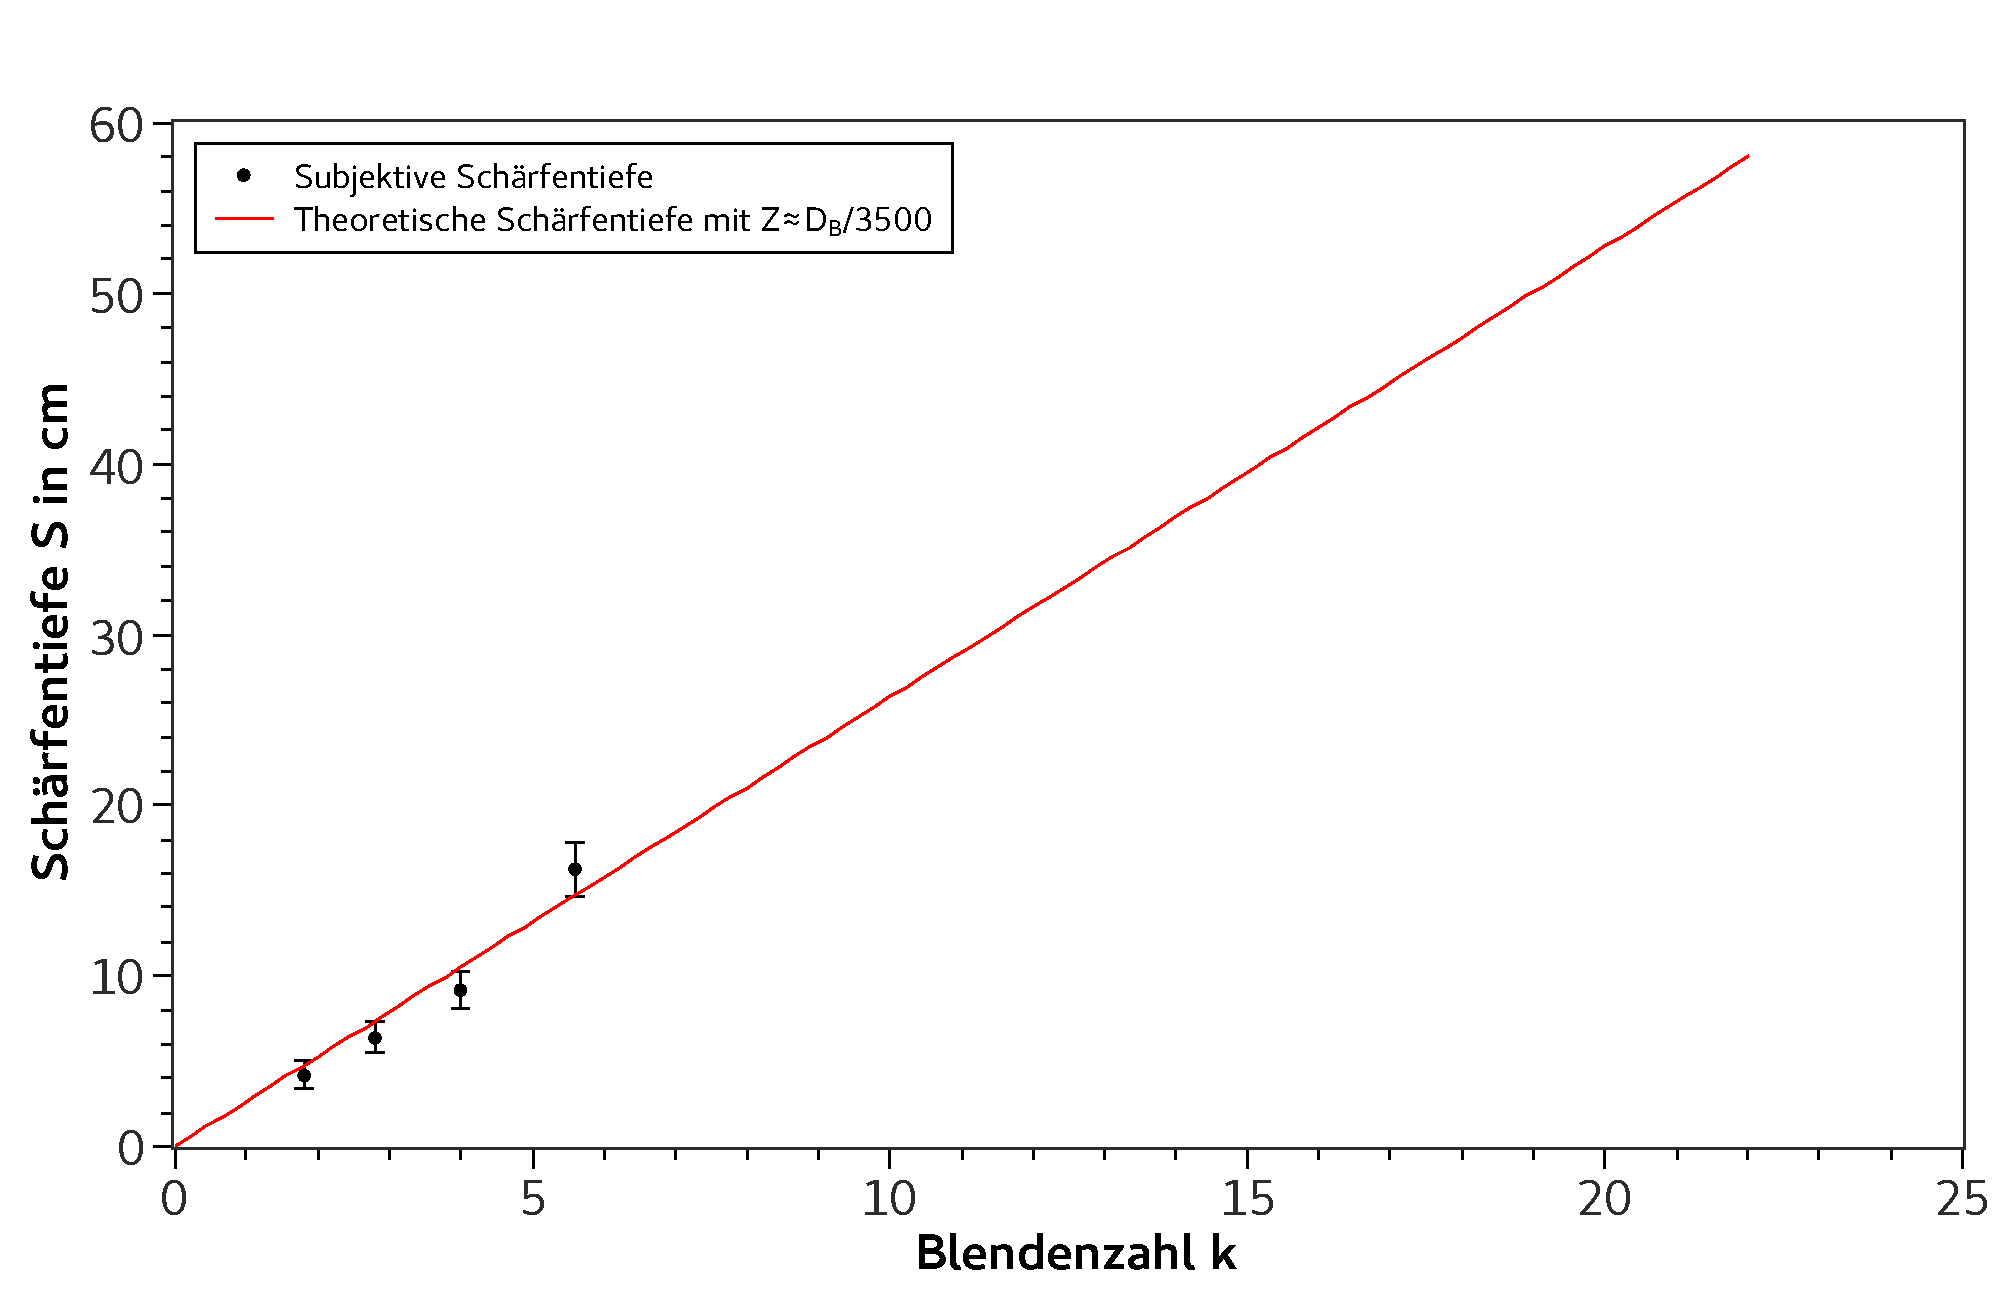
\includegraphics[width=1\textwidth]{fig_scharf_tief}
		\centering
		\caption{Die schwarzen Messpunkte sind die subjektiven Schärfentiefen, die noch mit der begrenzten Länge des Testcharts messbar waren.
			Die rote Funktion ist die theoretische Schärfentiefe nach \cref{eq_scharf_tief} mit entsprechenden Parametern.
			Die einzige Änderung, die durchgeführt wurde, ist die Skalierung der Durchmessergrenze $Z$ der Zerstreuungskreise mit einem Faktor von ca. 3/7.}
		\label{fig_scharf_tief}
		\centering
	\end{figure}

	Außergewöhnlich ist die hohe theoretische Schärfentiefe bei $k=22$ in \cref{tab_scharf_tief}.
	Der gesamte Verlauf der theoretischen Schärfentiefen ist in \cref{fig_scharf_tief_theo} abgebildet.
	Es ist auffällig, dass die Schärfentiefe bei $k\approx21$ sehr hohe Werte annimmt.
	Grund hierfür ist, dass der bei dieser Blendenzahl $d_h\approx g\approx\SI{64}{cm}$ ist.
	Die Definition des Fernpunkts \cref{eq_fernpunkt} besagt, dass dieser bei $g\geq d_h \Rightarrow d_f=\infty$.
	Daraus wiederum folgt nach $S=|d_h-d_f|$ eine sehr hohe Schärfentiefe.

	\begin{figure}[H]  
		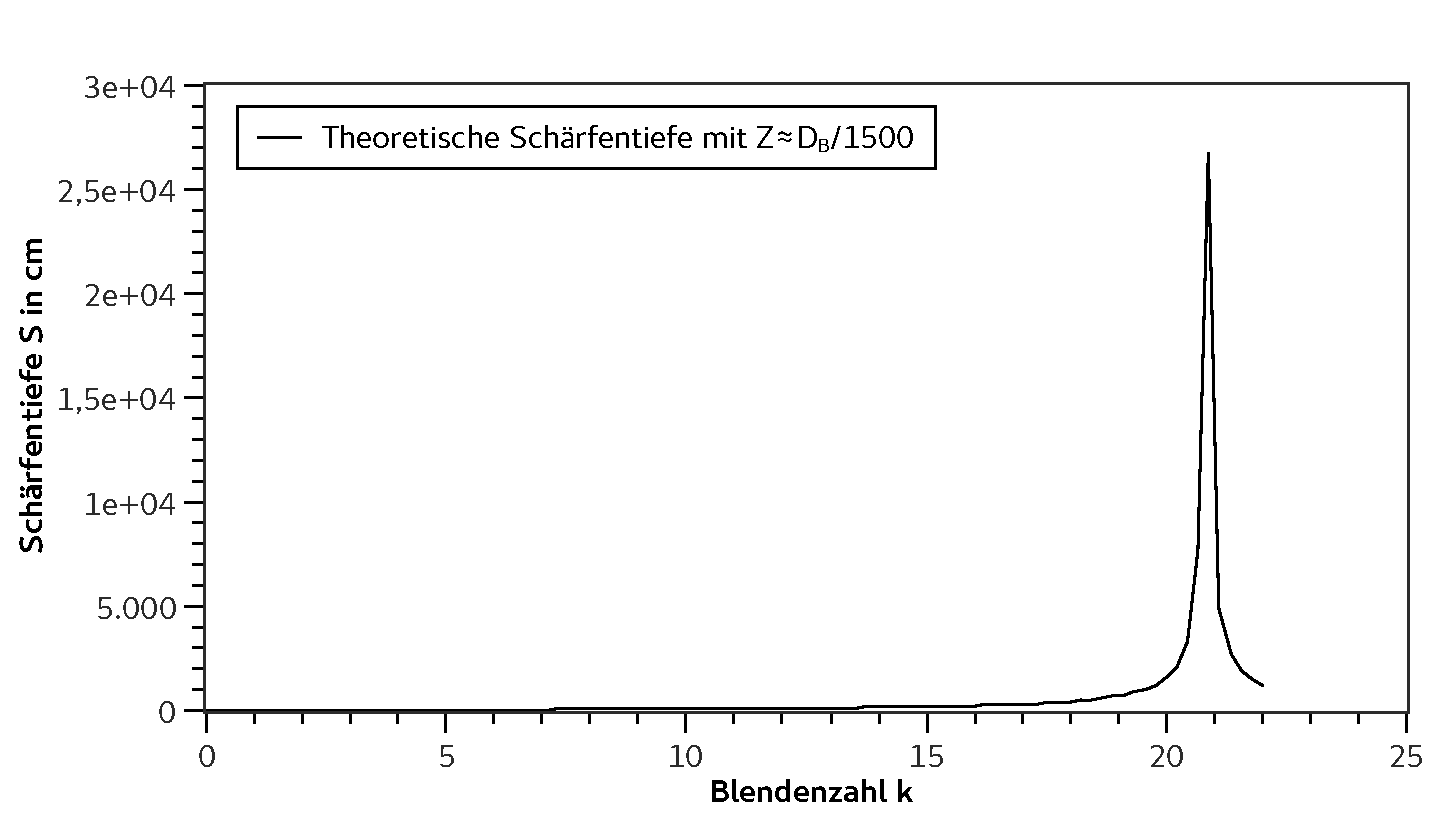
\includegraphics[width=1\textwidth]{fig_scharf_tief_theo}
		\centering
		\caption{
			Die schwarze Funktion ist theoretische Schärfentiefe nach \cref{eq_scharf_tief} mit entsprechenden Parametern.
			Die Schärfentiefe $S_\text{theo}$ wird sehr groß bei $k\approx21$.
			Dies entspricht dem Fall $g\approx d_h$, sodass $d_f$ divergiert.
			}
		\label{fig_scharf_tief_theo}
		\centering
	\end{figure}



	\subsection{Auflösung des Nikkor-Objektivs}
	\subsubsection{Beobachtung und Datenanalyse}
	
	Beim Fotografieren war das Testchart \SI{107,0+-0,81}{cm} von der Kamera entfernt und orthogonal ausgerichtet.
	Die MTF-Kurven, die sich mit dem ImageJ-Plugin berechnen lassen, sind in \cref{fig_schraeg_kante_mtf} dargestellt. 
	Es wird für alle Kurven ein Oversampling von 1 verwendet.
	Die resultierenden Halbwertsfrequenzen sind in \cref{fig_schraeg_kante} gegen die Blendenzahl aufgetragen.

	\begin{figure}[H]  
		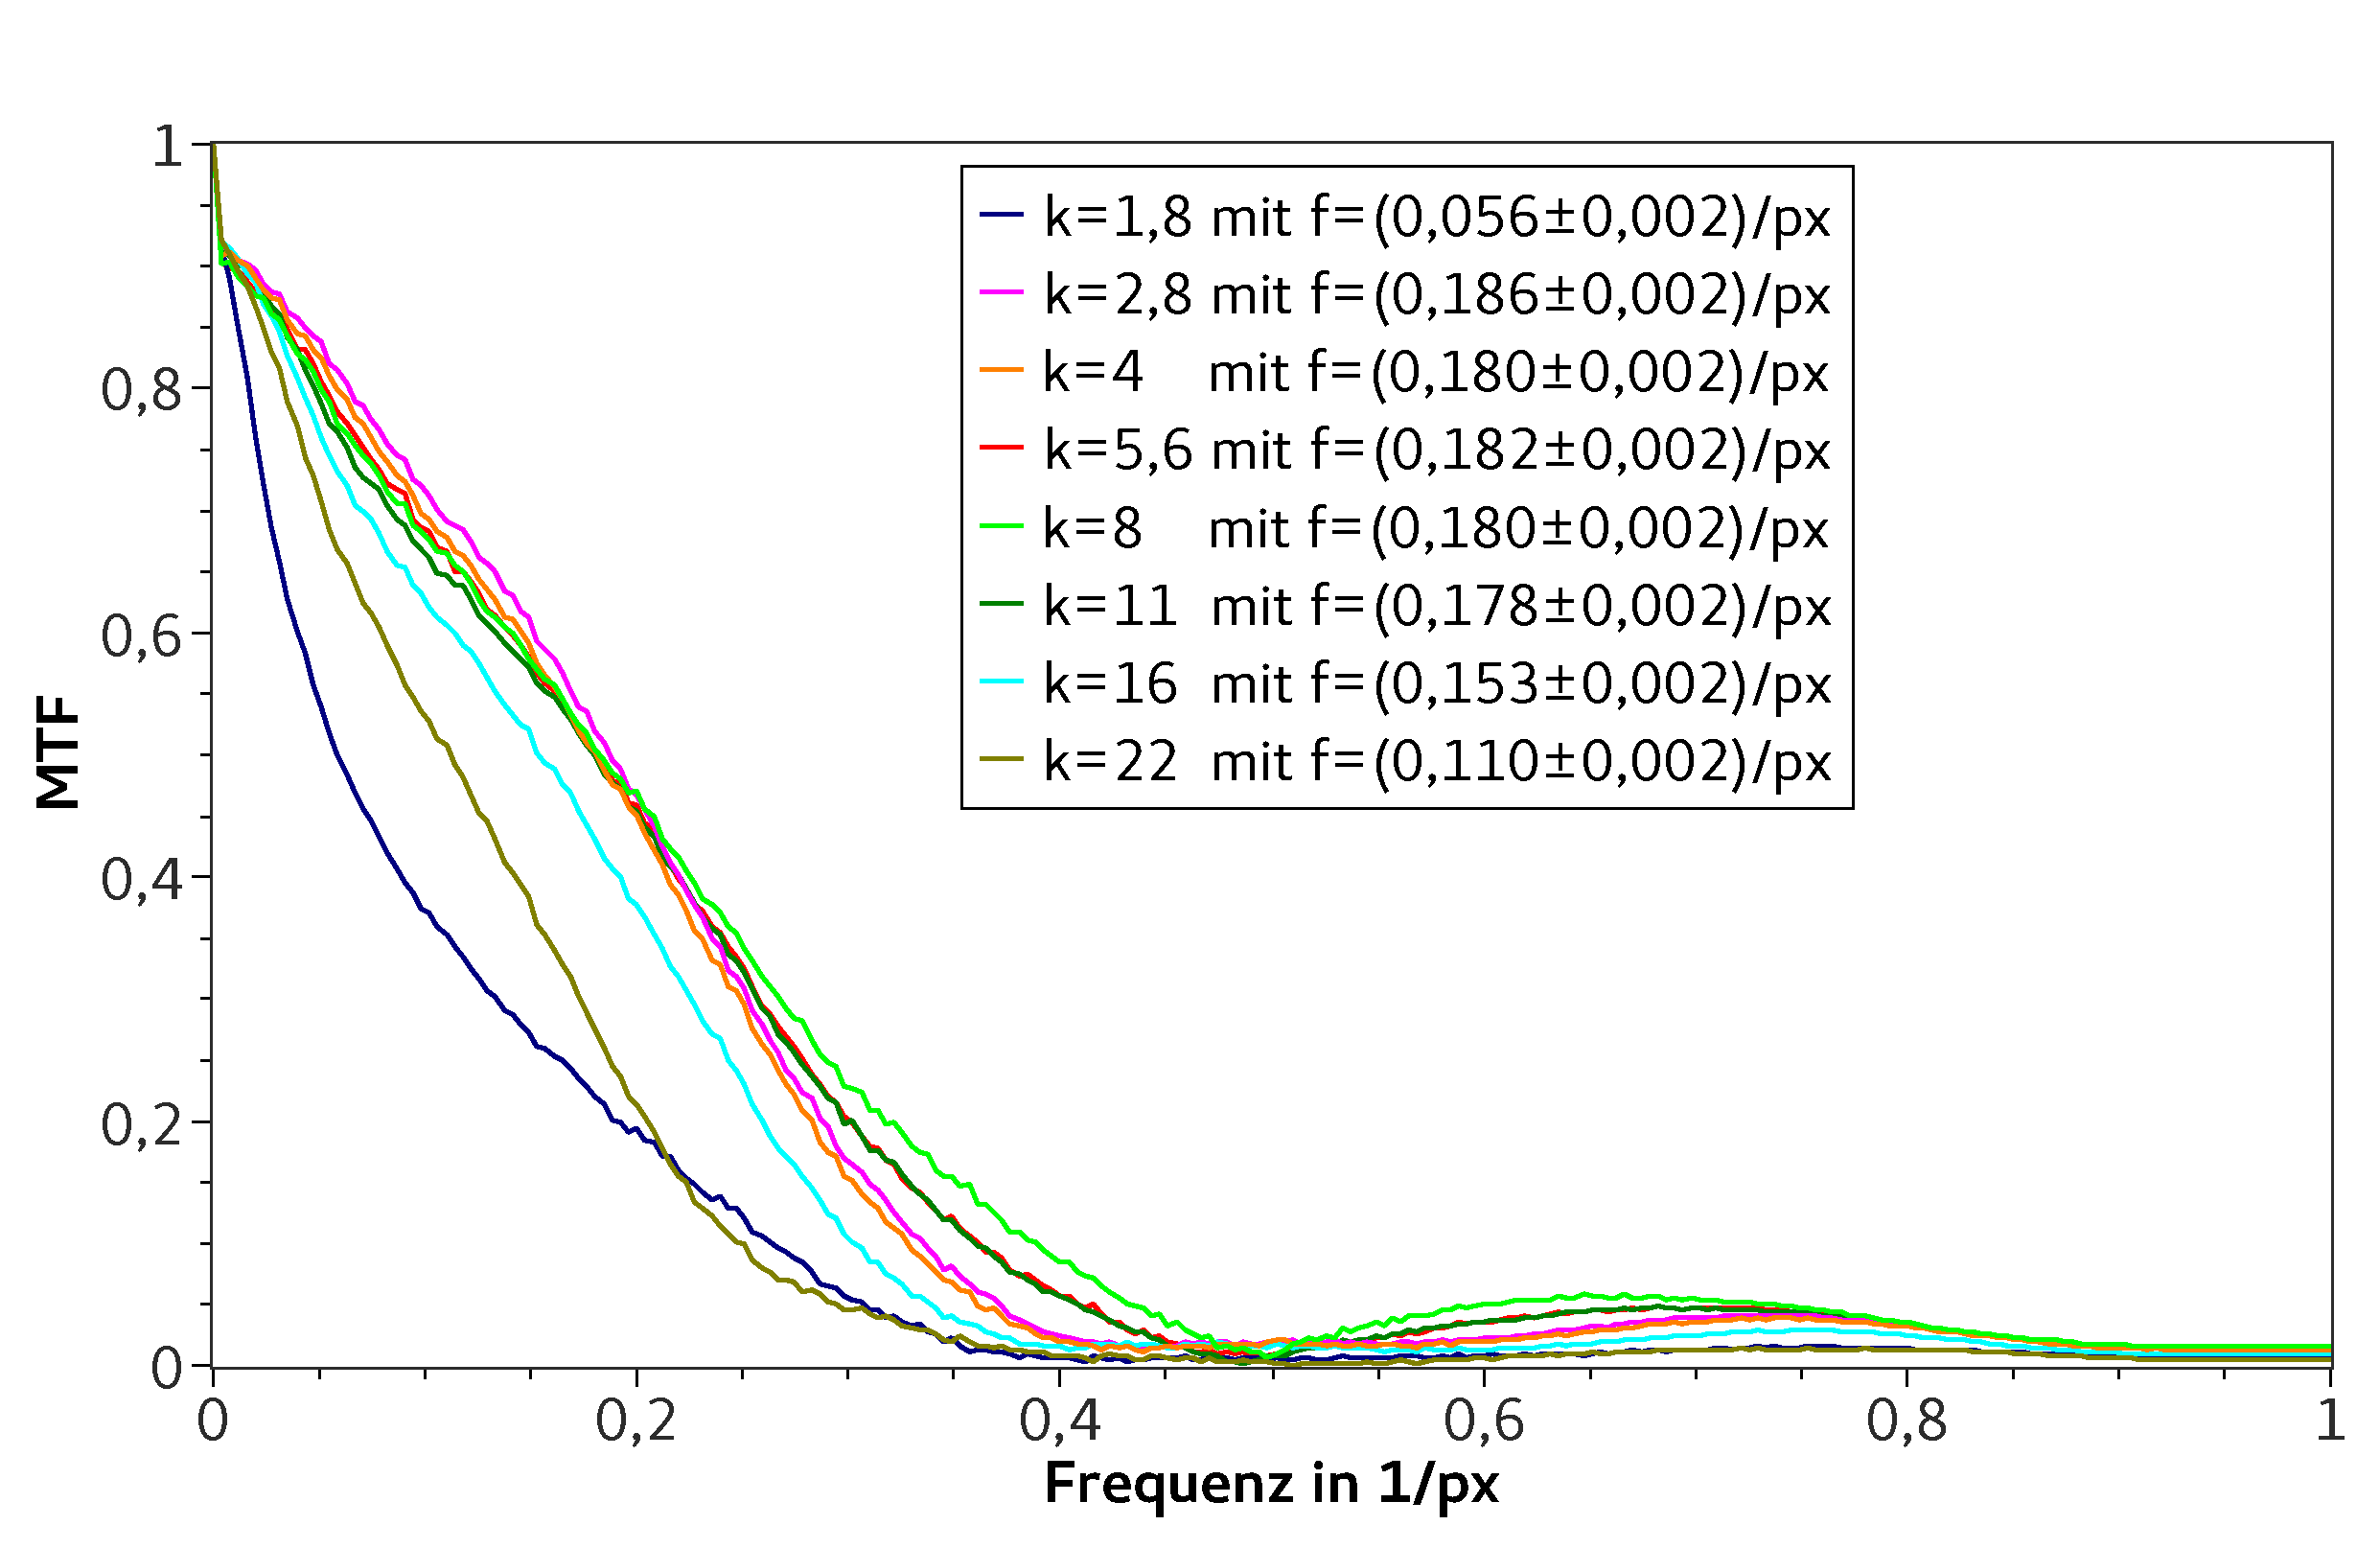
\includegraphics[width=1\textwidth]{fig_schraeg_kant_mtf}
		\centering
		\caption{
			MTF-Kurven der untersuchte Blendenzahlen $k$, die durch das ImageJ-Plugin "Praktikum Slanted Edge MTF" berechnet werden.
			Zur jeweiligen Funktion ist die Halbwertsfrequenz $f$ angegeben.
			}
		\label{fig_schraeg_kante_mtf}
		\centering
	\end{figure}

	\begin{figure}[H]  
		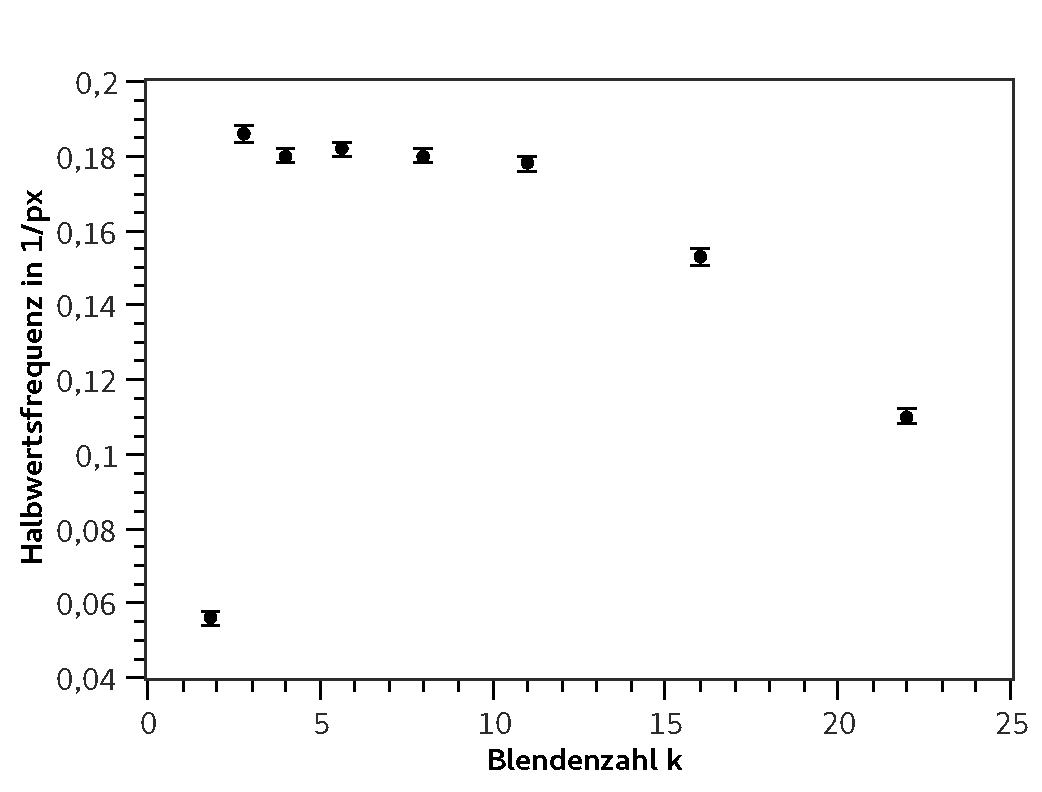
\includegraphics[width=1\textwidth]{fig_schraeg_kant_2}
		\centering
		\caption{
			Die Halbwertsfrequenz der MTFs aus \cref{fig_schraeg_kante_mtf} ist gegen die Blendenzahl aufgetragen.
			}
		\label{fig_schraeg_kante}
		\centering
	\end{figure}

	\subsubsection{Diskussion}
	Die beste Auflösung erhält man bei maximaler Halbwertsfrequenz, da scharfe Kanten nur durch hohe Frequenzen dargestellt werden können. 
	Wenn die die Halbwertsfrequenz gering ist, ist der Übergang ungenauer und "verschwommen".
	Folglich ist nach \cref{fig_schraeg_kante} die Auflösung des \SI{107}{cm} entfernten Testcharts am besten bei einer Blendenzahl $k$ von 2,8 bis 8.
	
	\subsection{Auflösung einer Einzellinse} \label{ss_einzellinse}
	\subsubsection{Beobachtung und Datenanalyse}
	Zunächst wird das Bild um den Faktor vier hochskaliert, um Interpolationsungenauigkeiten bei der Erstellung der Linienprofile zu vermeiden.
	Dann wird jeweils eine Achse durch zwei gegenüberliegende schwarze und zwei gegenüberliegende weiße Bereiche des Siemenssterns gezogen und ein Linienprofil der Grauwerte erstellt.
	Die beiden Profile werden übereinander gelegt, sodass die Grauwerte am grauen Rand des Siemenssterns und die Maxima in der weißen Mitte  übereinander liegen.
	Als Beispiel ist eine Überlagerung dieser Profile in \cref{fig_einzel_linie} dargestellt.
	Dann wird, um den Durchmesser der grauen Fläche in der Mitte der Aufnahme des Siemenssterns in Pixeln zu bestimmen, der Schnittpunkt der beiden Graphen, ab dem die Profile näherungsweise gleich verlaufen, auf beiden Seiten der Mitte abgelesen.
	Dies erlaubt die Umrechnung des Durchmessers der grauen Fläche von Pixeln in Meter, da bekannt ist, dass der weiße Innenkreis einen Durchmesser von \SI{1,5}{mm} hat.
	Diese Angabe sowie die Durchmesser der Blenden werden als exakt angenommen.
	Die Unsicherheit beim richtigen Überlagern der Kurven und Ablesen der Schnittpunkte wird mit \SI{30}{px} abgeschätzt.
	Für die Differenz der Schnittpunkte ergibt sich somit gemäß GUM $u(d)= \SI{43}{px}$.
	Da bei manchen Blendendurchmessern aufgrund der hohen Asymmetrie das Ablesen der Schnittpunkte nicht eindeutig war, wurde dort der doppelte Fehler verwendet.
	Die Breite der Mitte ist meistens deutlich eindeutiger ablesbar, weshalb hier eine Unsicherheit von \SI{13}{px} aufgrund der geringen Schwankung des eigentlich als konstant erwarteten Wertes (bei konstantem Abstand der Kamera vom Schirm) angenommen wird.
	
	\begin{figure}[H]  
		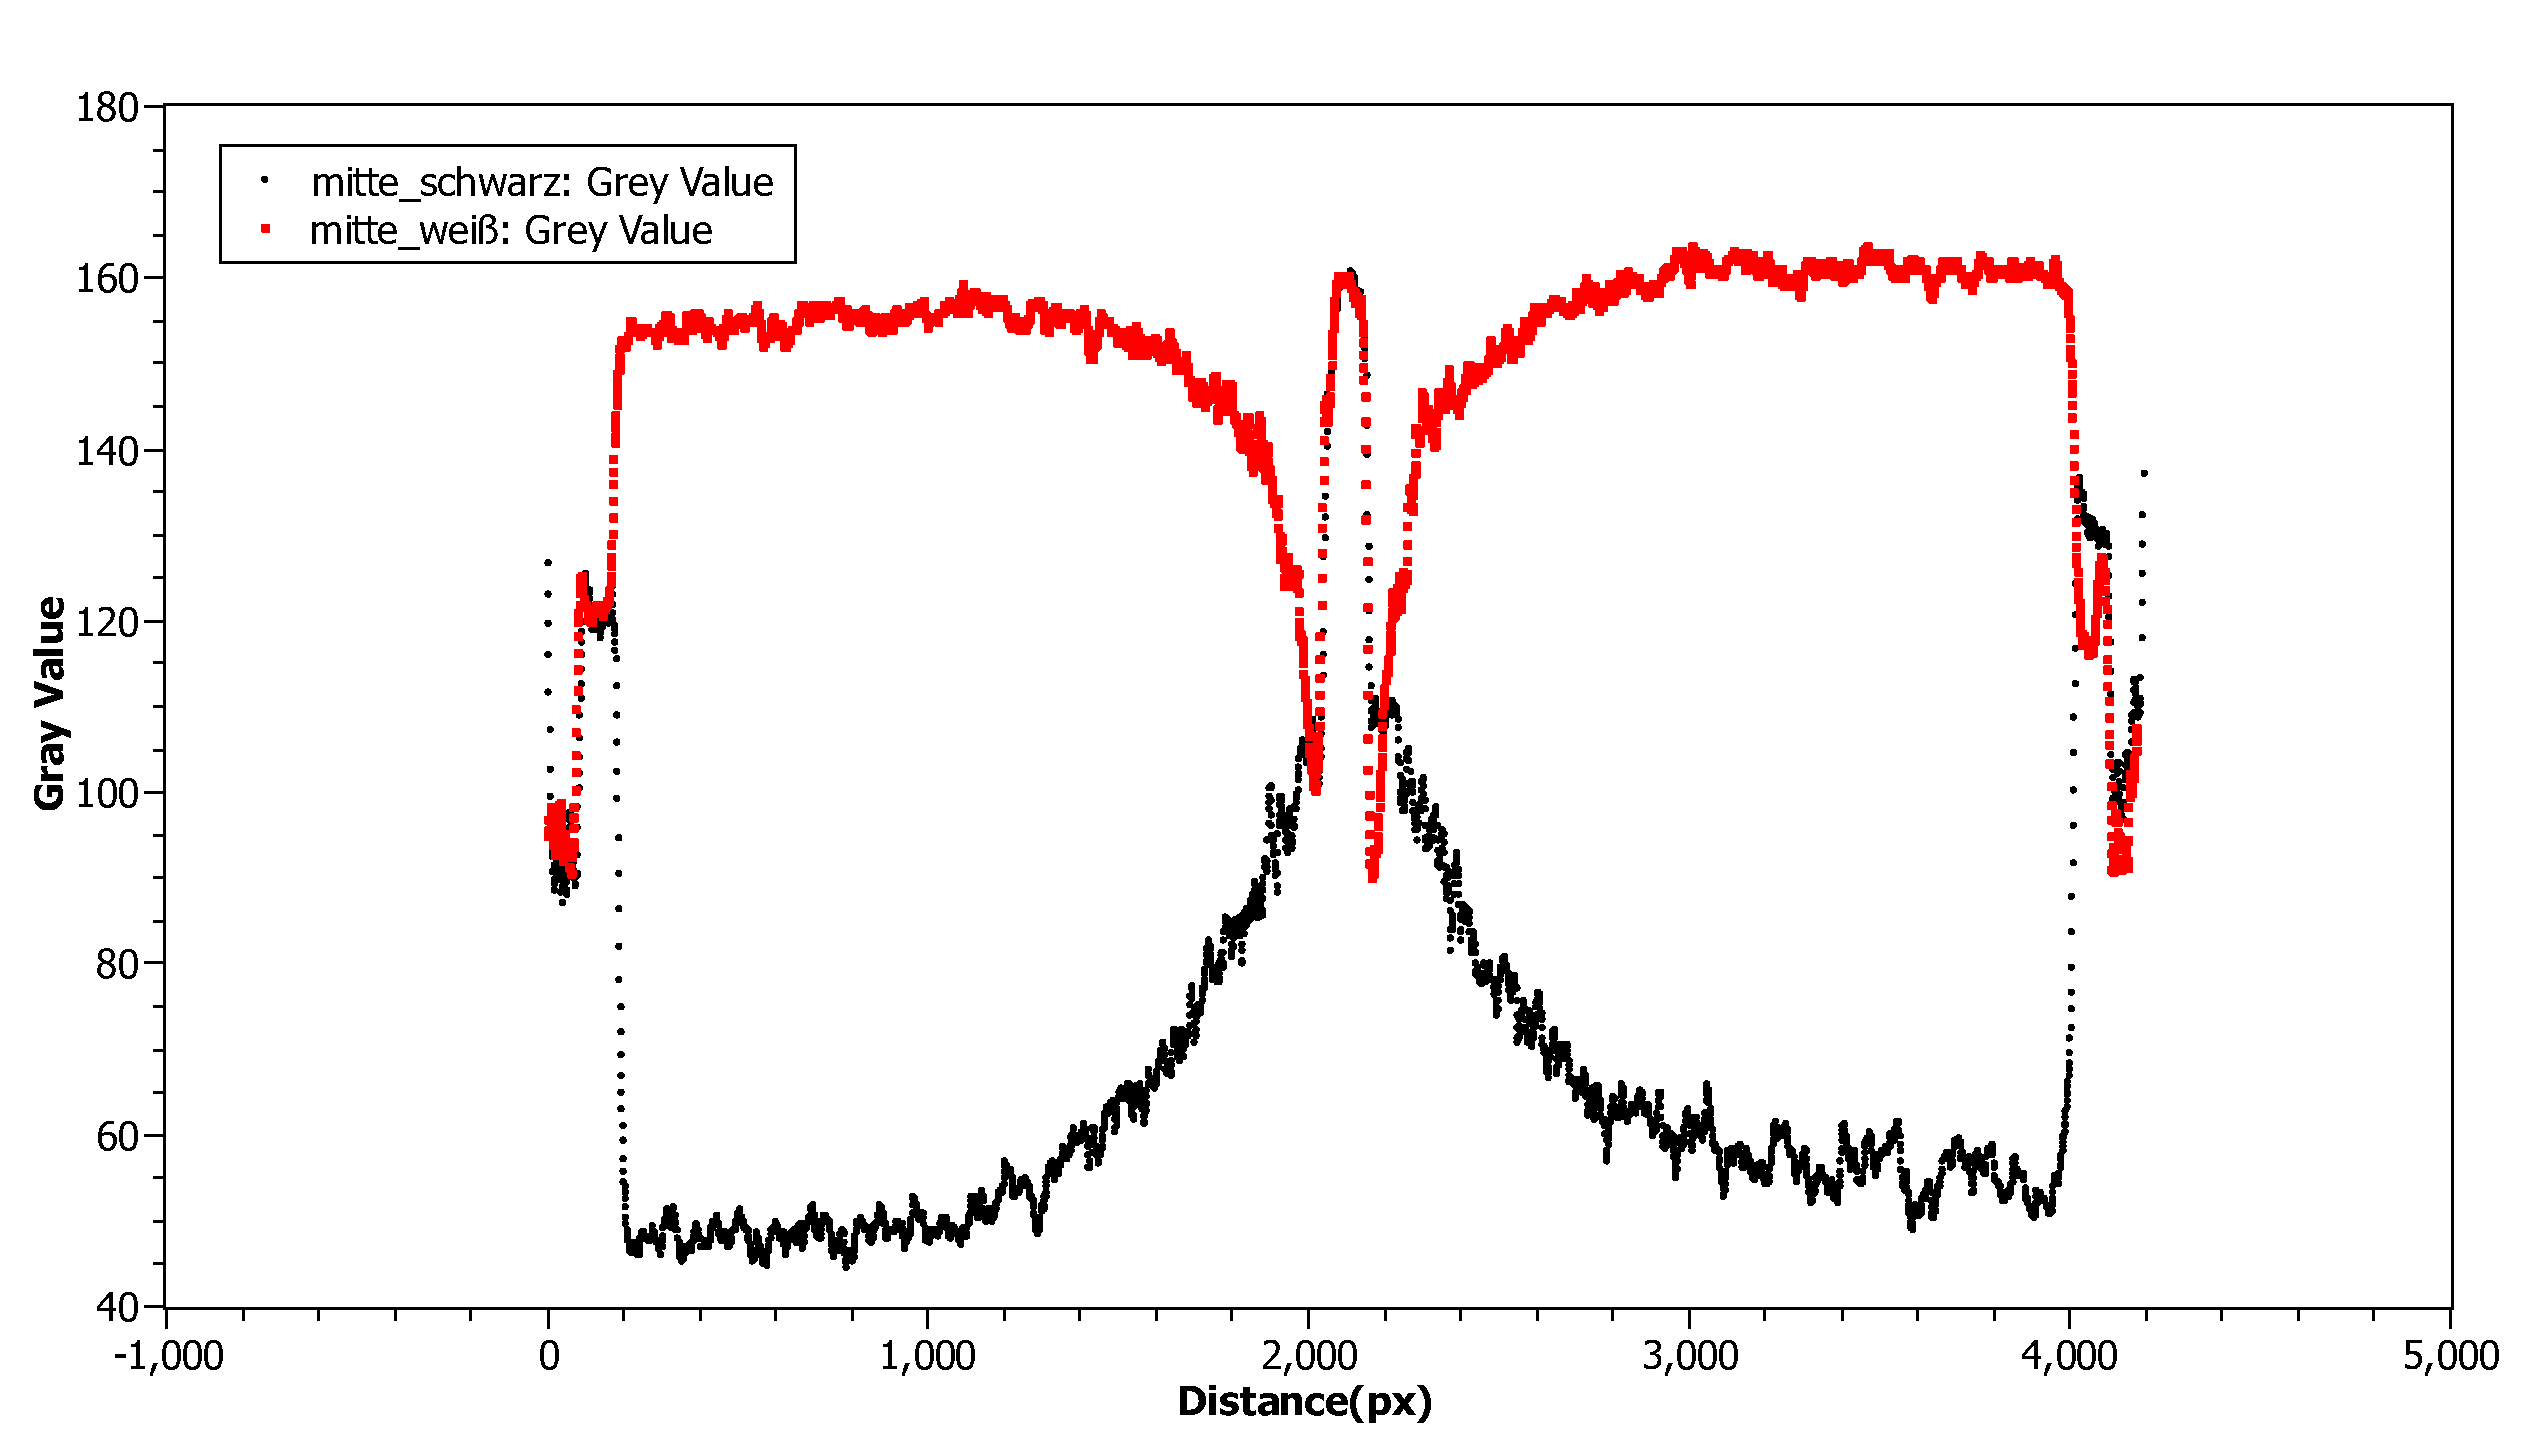
\includegraphics[width=1\textwidth]{fig_Einzellinse_Linienprofil}
		\centering
		\caption{
			Überlagerung der Linienprofile von schwarzem zu schwarzem bzw. weißem zu weißem Bereich des Siemenssterns.
			Abgelesen werden der Abstand der Schnittpunkte der Profile in der Mitte sowie die Breite des Maximums in der Mitte.
			Ein Wert von 0 entspricht dabei Schwarz und ein Wert von 255 entspricht Weiß.
		}
		\label{fig_einzel_linie}
		\centering
	\end{figure}
	
	Die Umrechnung der Breite $d$ der grauen Fläche in \si{mm} erfolgt gemäß:
	\begin{equation}
		d = \frac{\SI{1,5}{mm} \cdot b}{m}
	\end{equation}
	Dabei ist $b$ die Breite $d$ in Pixeln und $m$ die Breite des weißen, \SI{1,5}{mm} breiten Bereichs in der Mitte.
	Dass das Bild mit dem Faktor 4 hochskaliert wurde spielt hier keine Rolle, da dieser Faktor sowohl in $m$ als auch in $b$ einfließt und durch den Bruch wegfällt.
	Die Unsicherheit ergibt sich gemäß:
	\begin{equation}
		u(d)=\sqrt{\left(\frac{\SI{1,5}{mm} \cdot b \cdot u(m)}{m^2}\right)^2+\left(\frac{\SI{1,5}{mm} \cdot u(b)}{m}\right)^2}
	\end{equation}
	
	Für die Auflösung in Linienpaaren $l$ gilt
	\begin{equation}
		l=\frac{\pi d}{n}
	\end{equation}
	mit der Unsicherheit
	\begin{equation}
		u(l)=\left|\frac{\pi u(d)}{n}\right|.
	\end{equation}
	
	Das Ergebnis aus dieser Rechnung für den Siemensstern am Rand der Fotografie ist in \cref{fig_aufl} dargestellt.
	
	\begin{figure}[H]
		\centering
		\begin{subfigure}[t]{0.5\textwidth}
			\centering
			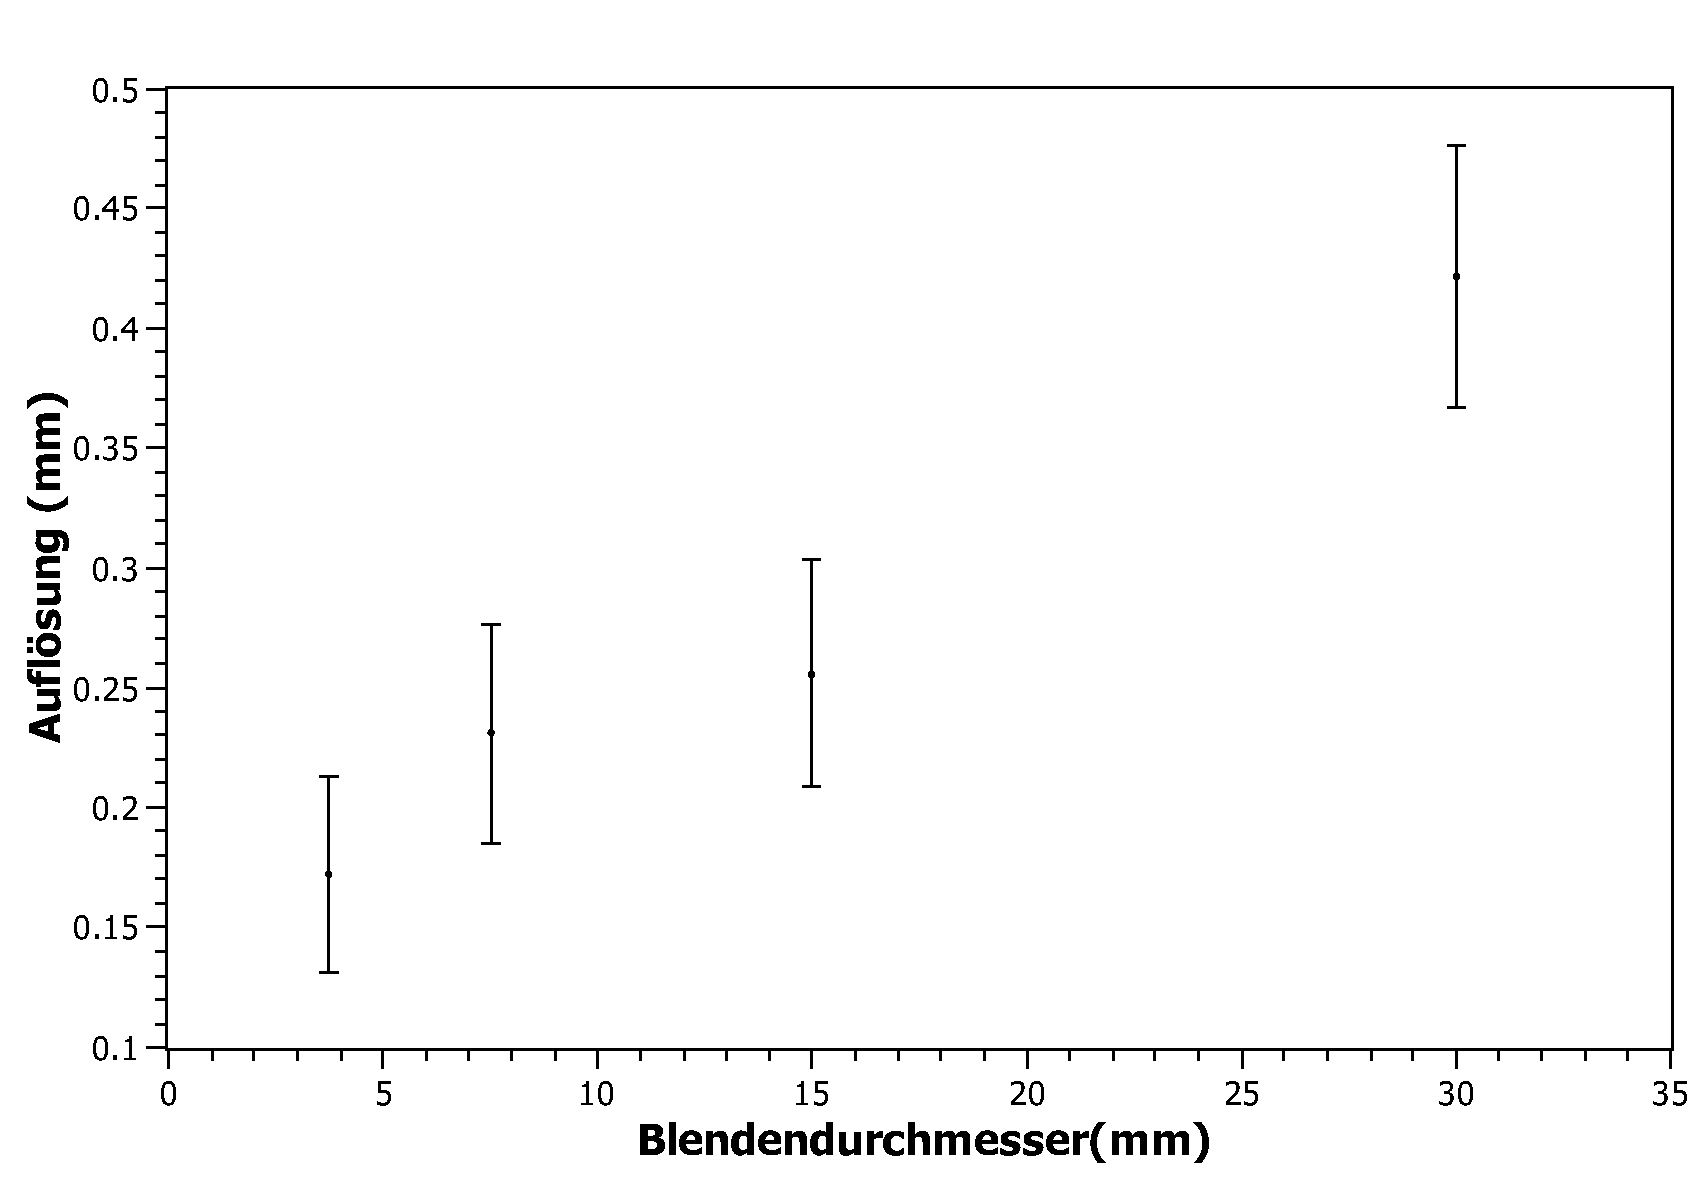
\includegraphics[width=1\textwidth]{fig_Einzellinse_mitte_aufloesung}
			\label{fig_aufl_mitte}
			\caption{Mitte}
		\end{subfigure}%
		\begin{subfigure}[t]{0.5\textwidth}
			\centering
			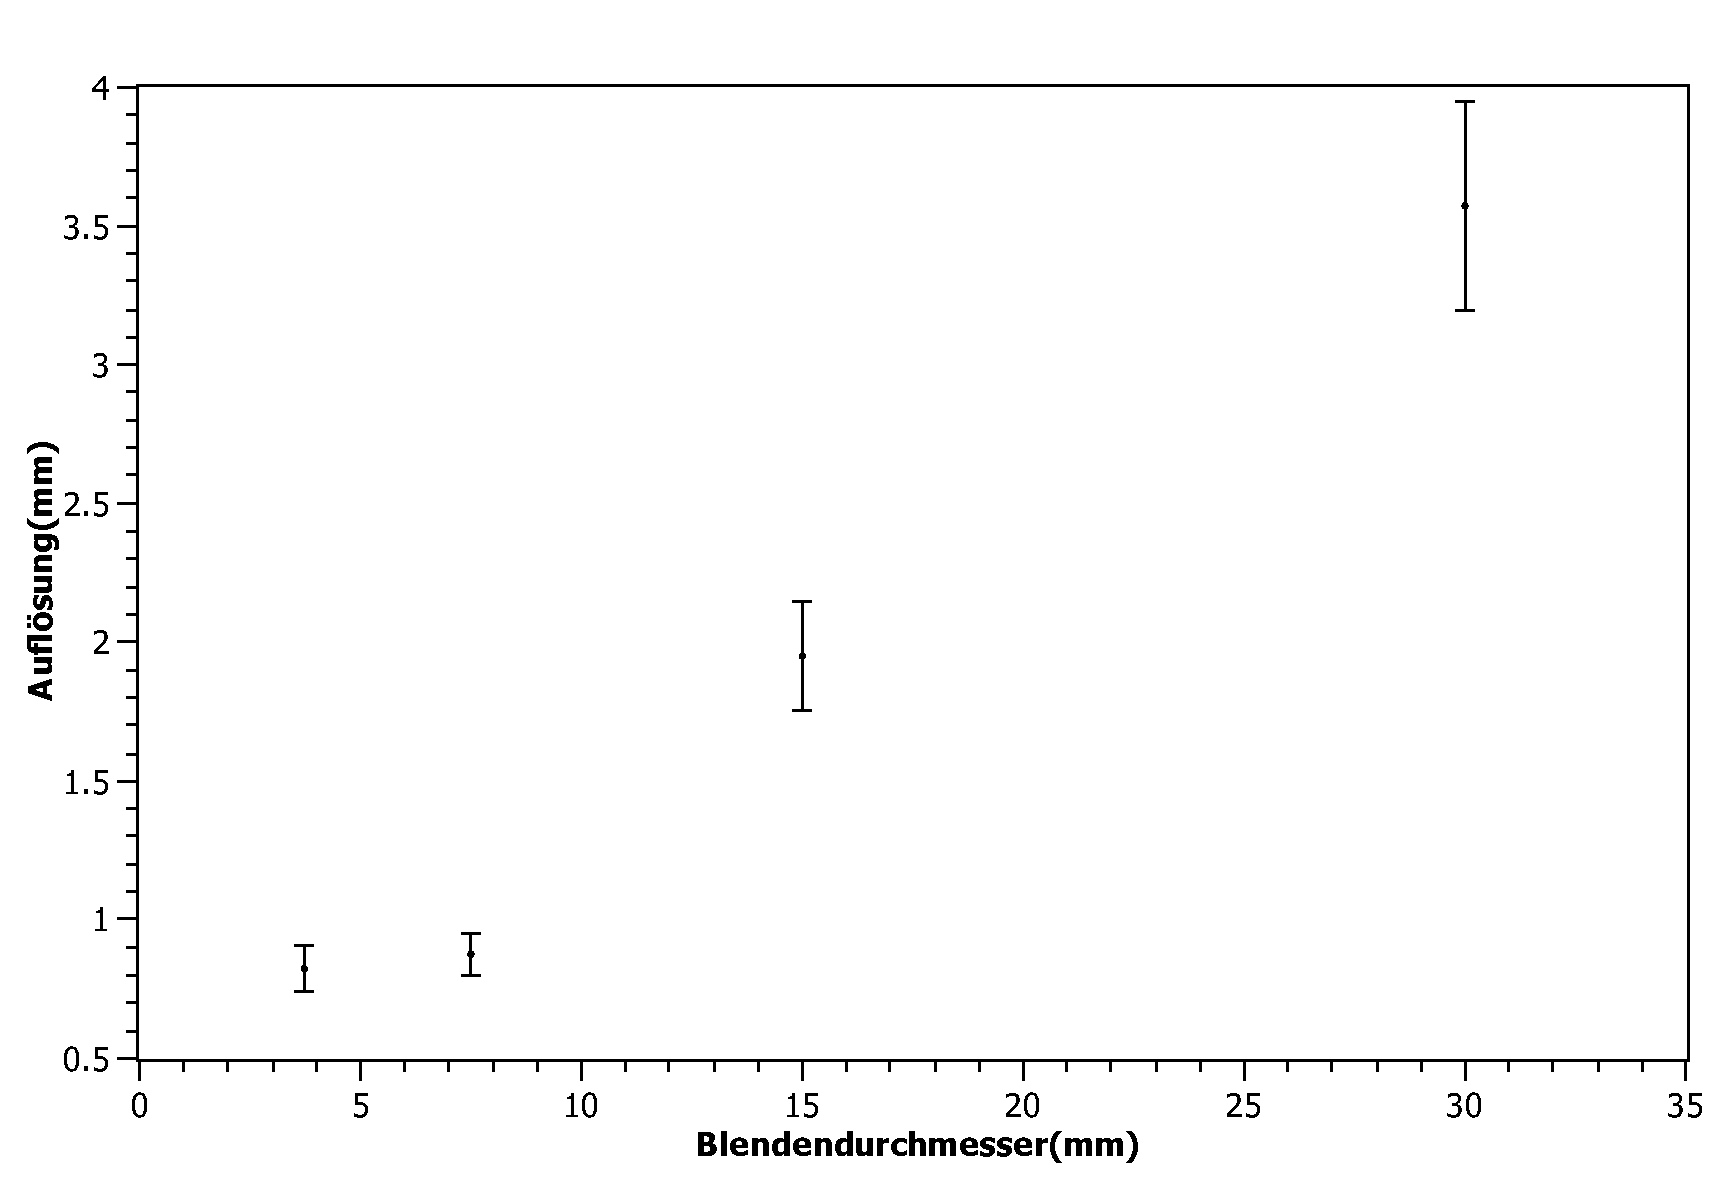
\includegraphics[width=1\textwidth]{fig_Einzellinse_rand_aufloesung}
			\label{fig_aufl_rand}
			\caption{Rand}
		\end{subfigure}
		\caption{
			\label{fig_aufl}
			Auflösung in Linienpaaren der Kamera mit Einzellinse bei verschiedenen Blendendurchmessern am Rand und in der Mitte der Fotografie.}
		\centering
		
	\end{figure}
	
	Zusätzlich wird für die vier Bilder des Testcharts mit unterschiedlichen Blendendurchmessern die MTF-Kurve  mit dem ImageJ-Plugin berechnet und die Halbwertsfrequenz abgelesen.
	Das Ergebnis ist in \cref{fig_einzel_mtf} abgebildet.
	
	\begin{figure}[H]  
		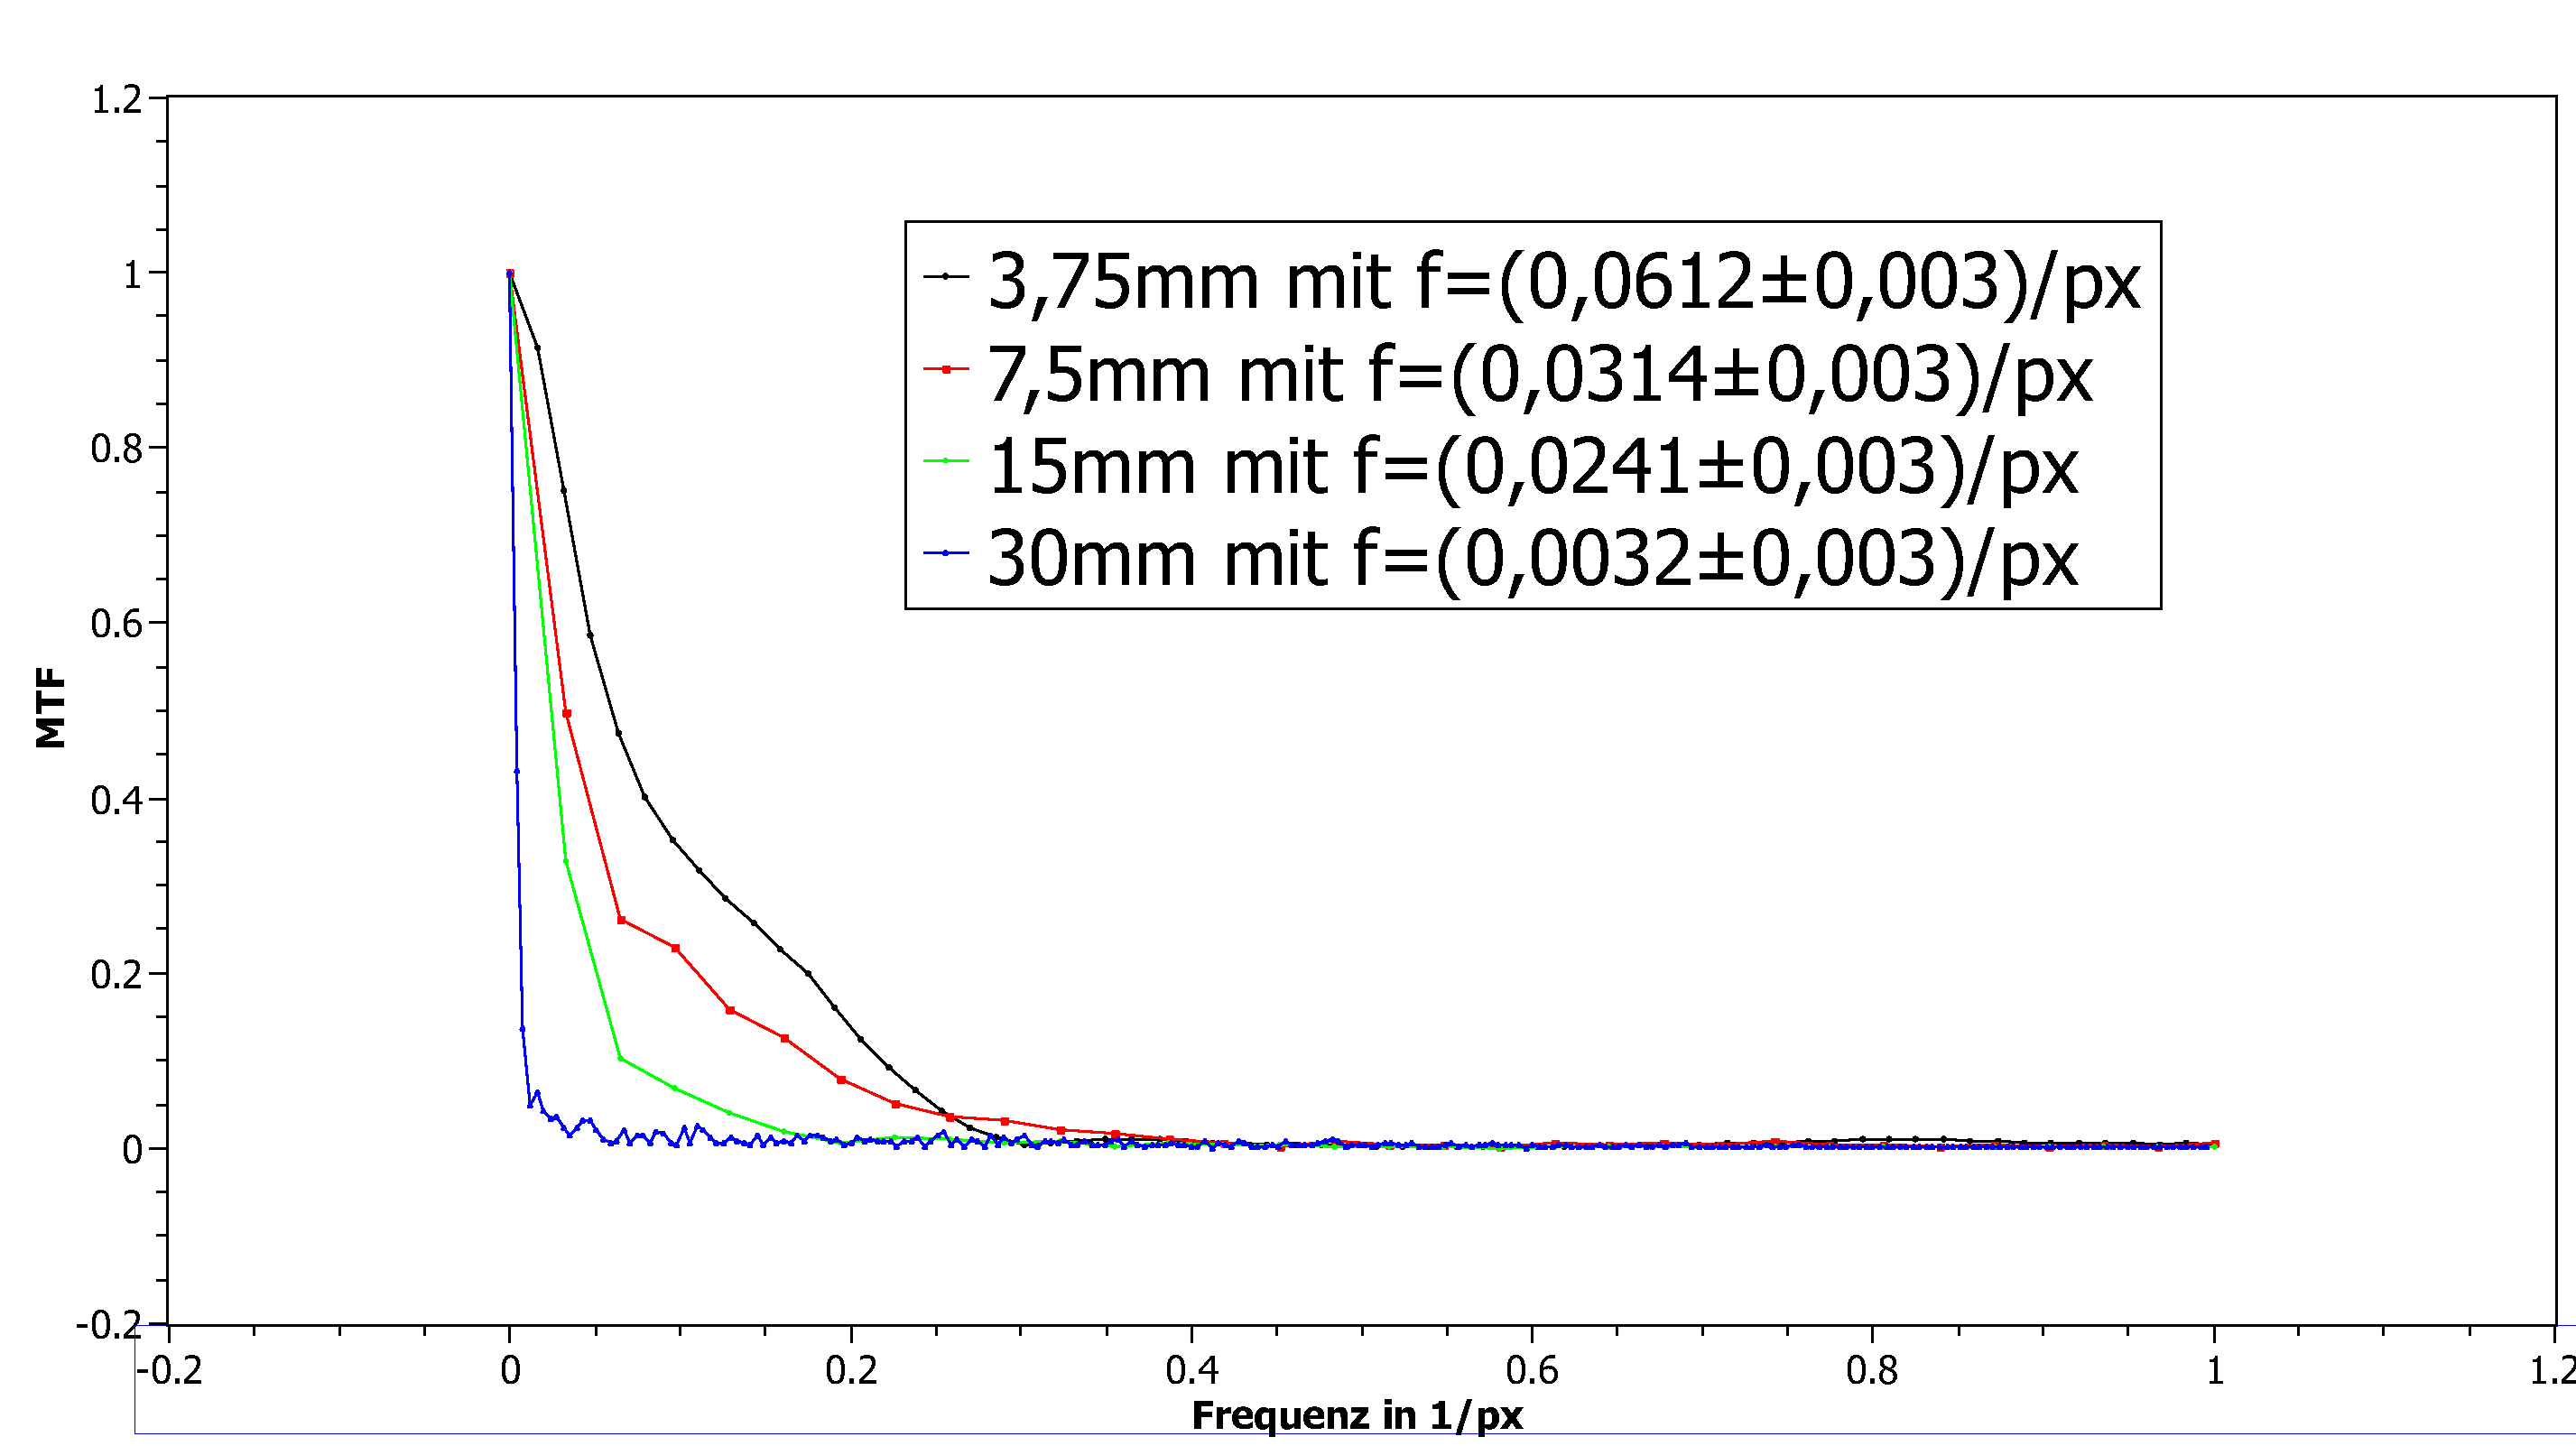
\includegraphics[width=1\textwidth]{fig_Einzellinse_MTF}
		\centering
		\caption{
			MTF-Kurven der Einzellinse bei unterschiedlichen Blendendurchmessern, die durch das ImageJ-Plugin "Praktikum Slanted Edge MTF" berechnet wurden.
			Die Messpunkte sind durch Linien verbunden, um die Interpolation zu erleichtern. %ganz ganz theoretisch nicht erlaubt, aber wenn der Mensch denken kann, ist klar, dass das nicht anders geht.
			Zur jeweiligen Funktion ist die Halbwertsfrequenz $f$ angegeben.
		}
		\label{fig_einzel_mtf}
		\centering
	\end{figure}
	

	\subsubsection{Diskussion}
	Offensichtlich wird zunächst, dass die Auflösung mit dem Blendendurchmesser steigt, während die Halbwertsfrequenz mit dem Blendendurchmesser sinkt, da bei kleinen Blendendurchmessern weniger nicht achsenparallele Strahlen auf die Linse treffen.
	Es fällt auf, dass die Profile nicht immer, wie zu erwarten war, achsensymmetrisch zur Mitte sind.
	Dies lässt sich auf Linsenfehler zurückführen, die dazu führen, dass achsenfernere Strahlen nicht gleich abgebildet werden wie achsennahe.
	Dies lässt sich dadurch bestätigen, dass dies bei den Linienprofilen des Siemenssterns am Rande der Fotografie deutlich stärker auffällt als bei dem nahe der Mitte, was auch durch die im Allgemeinen geringere Auflösung am Siemensstern am Rand unterstützt wird.
	
	In \cref{fig_einzel_vgl} ist die Halbwertsfrequenz aus den MTF-Kurven gegen den Kehrwert der Auflösung in Linienpaaren aufgetragen, wobei sich aus jedem Blendendurchmesser ein Punkt ergibt.
	Dabei wird nur der Siemensstern nahe der Mitte des Bildes verwendet.
	Zu erwarten ist hier ein linearer Zusammenhang, wobei die Steigung des Graphen dem Umrechnungsfaktor von Pixel zu Millimeter entsprechen sollte, der gemäß der Bestimmung des Durchmessers des Mittelpunkts der Siemenssterne etwa
	
	\begin{equation*}
		 \frac{\SI{1,5}{mm}}{\SI{142}{px}} \approx \SI{0,011}{mm/px} %TODO Unsicherheit maybe
	\end{equation*}
	beträgt.
	Um dies zu überprüfen wurde ein linearer Fit durchgeführt.
	Dieser ergibt für die Steigung einen Faktor von \SI{0,017\pm 0,002}{mm}.
	Die Vermutung, dass sich aus dem Kehrwert der Auflösung mit dem Umrechnungsfaktor von Pixeln zu Millimeter die Halbwertsfrequenz der MTF-Kurve bestimmen lässt, kann also nur größenordnungsmäßig bestätigt werden.
	Der lineare Zusammenhang lässt sich jedoch sehr eindeutig erkennen.
	
	\begin{figure}[H]  
		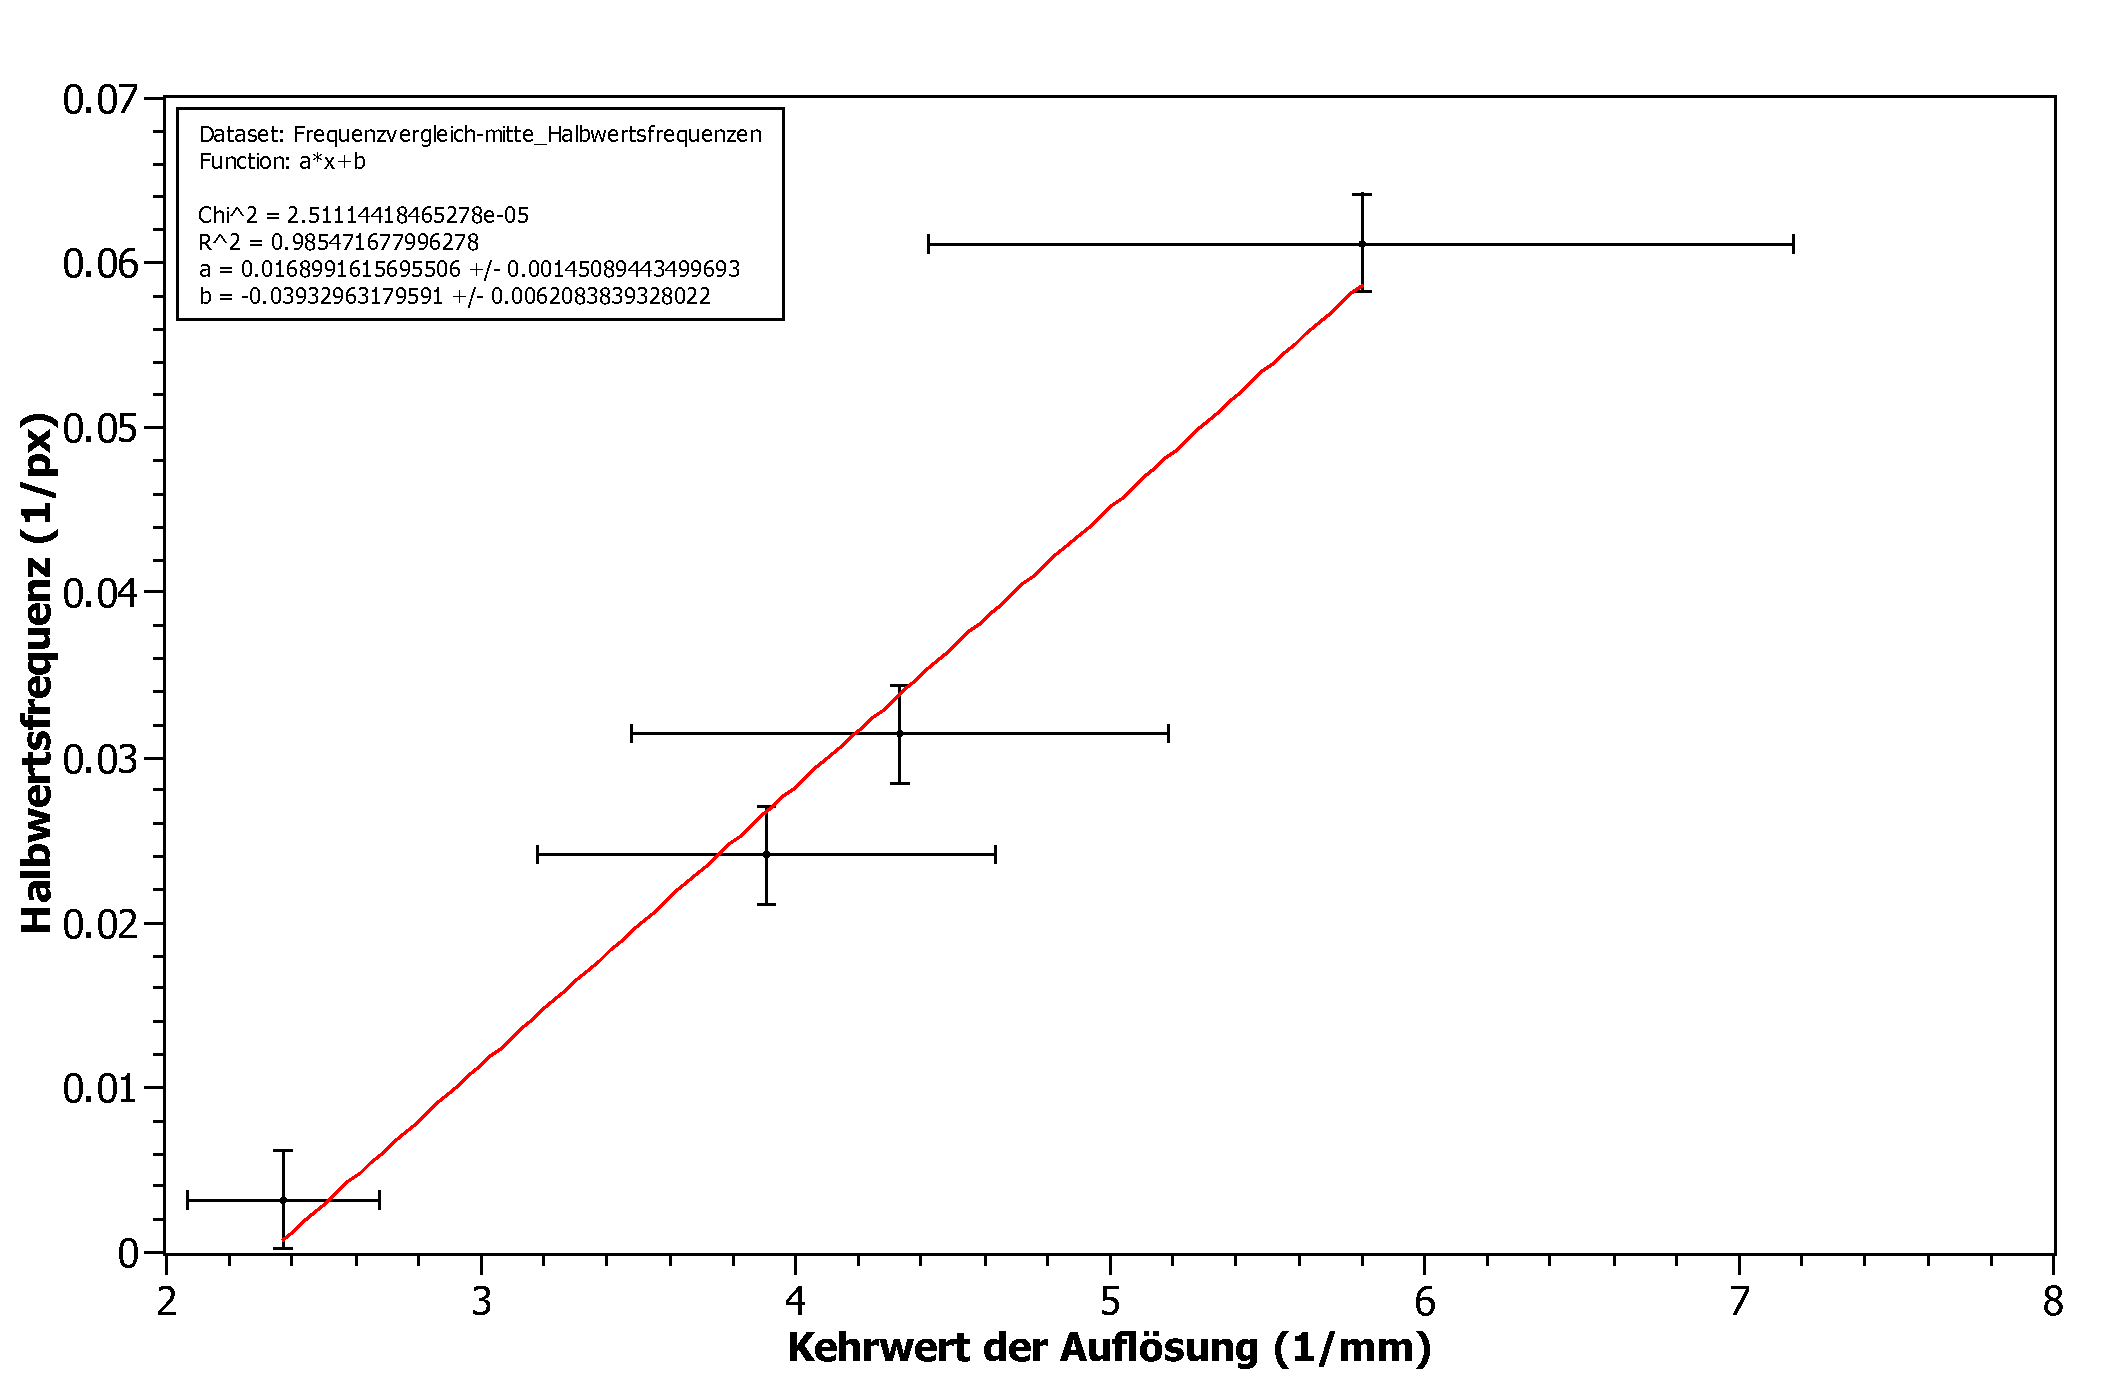
\includegraphics[width=1\textwidth]{fig_Einzellinse_Vergleich}
		\centering
		\caption{
			Es ist die Halbwertsfrequenz gegen den Kehrwert der Auflösung in Linienpaaren $l$ bei gleichem Blendendurchmesser aufgetragen.
			Es wurde ein linearer Fit durchgeführt, der in rot dargestellt ist.
		}
		\label{fig_einzel_vgl}
		\centering
	\end{figure}
	
	\subsection{Auflösung der Lochblende}
	\subsubsection{Beobachtung und Datenanalyse}
	Analog zur Einzellinse werden die Linienprofile des Siemenssterns erstellt und in \cref{fig_lochblende_profil} dargestellt.
	
	\begin{figure}[H]  
		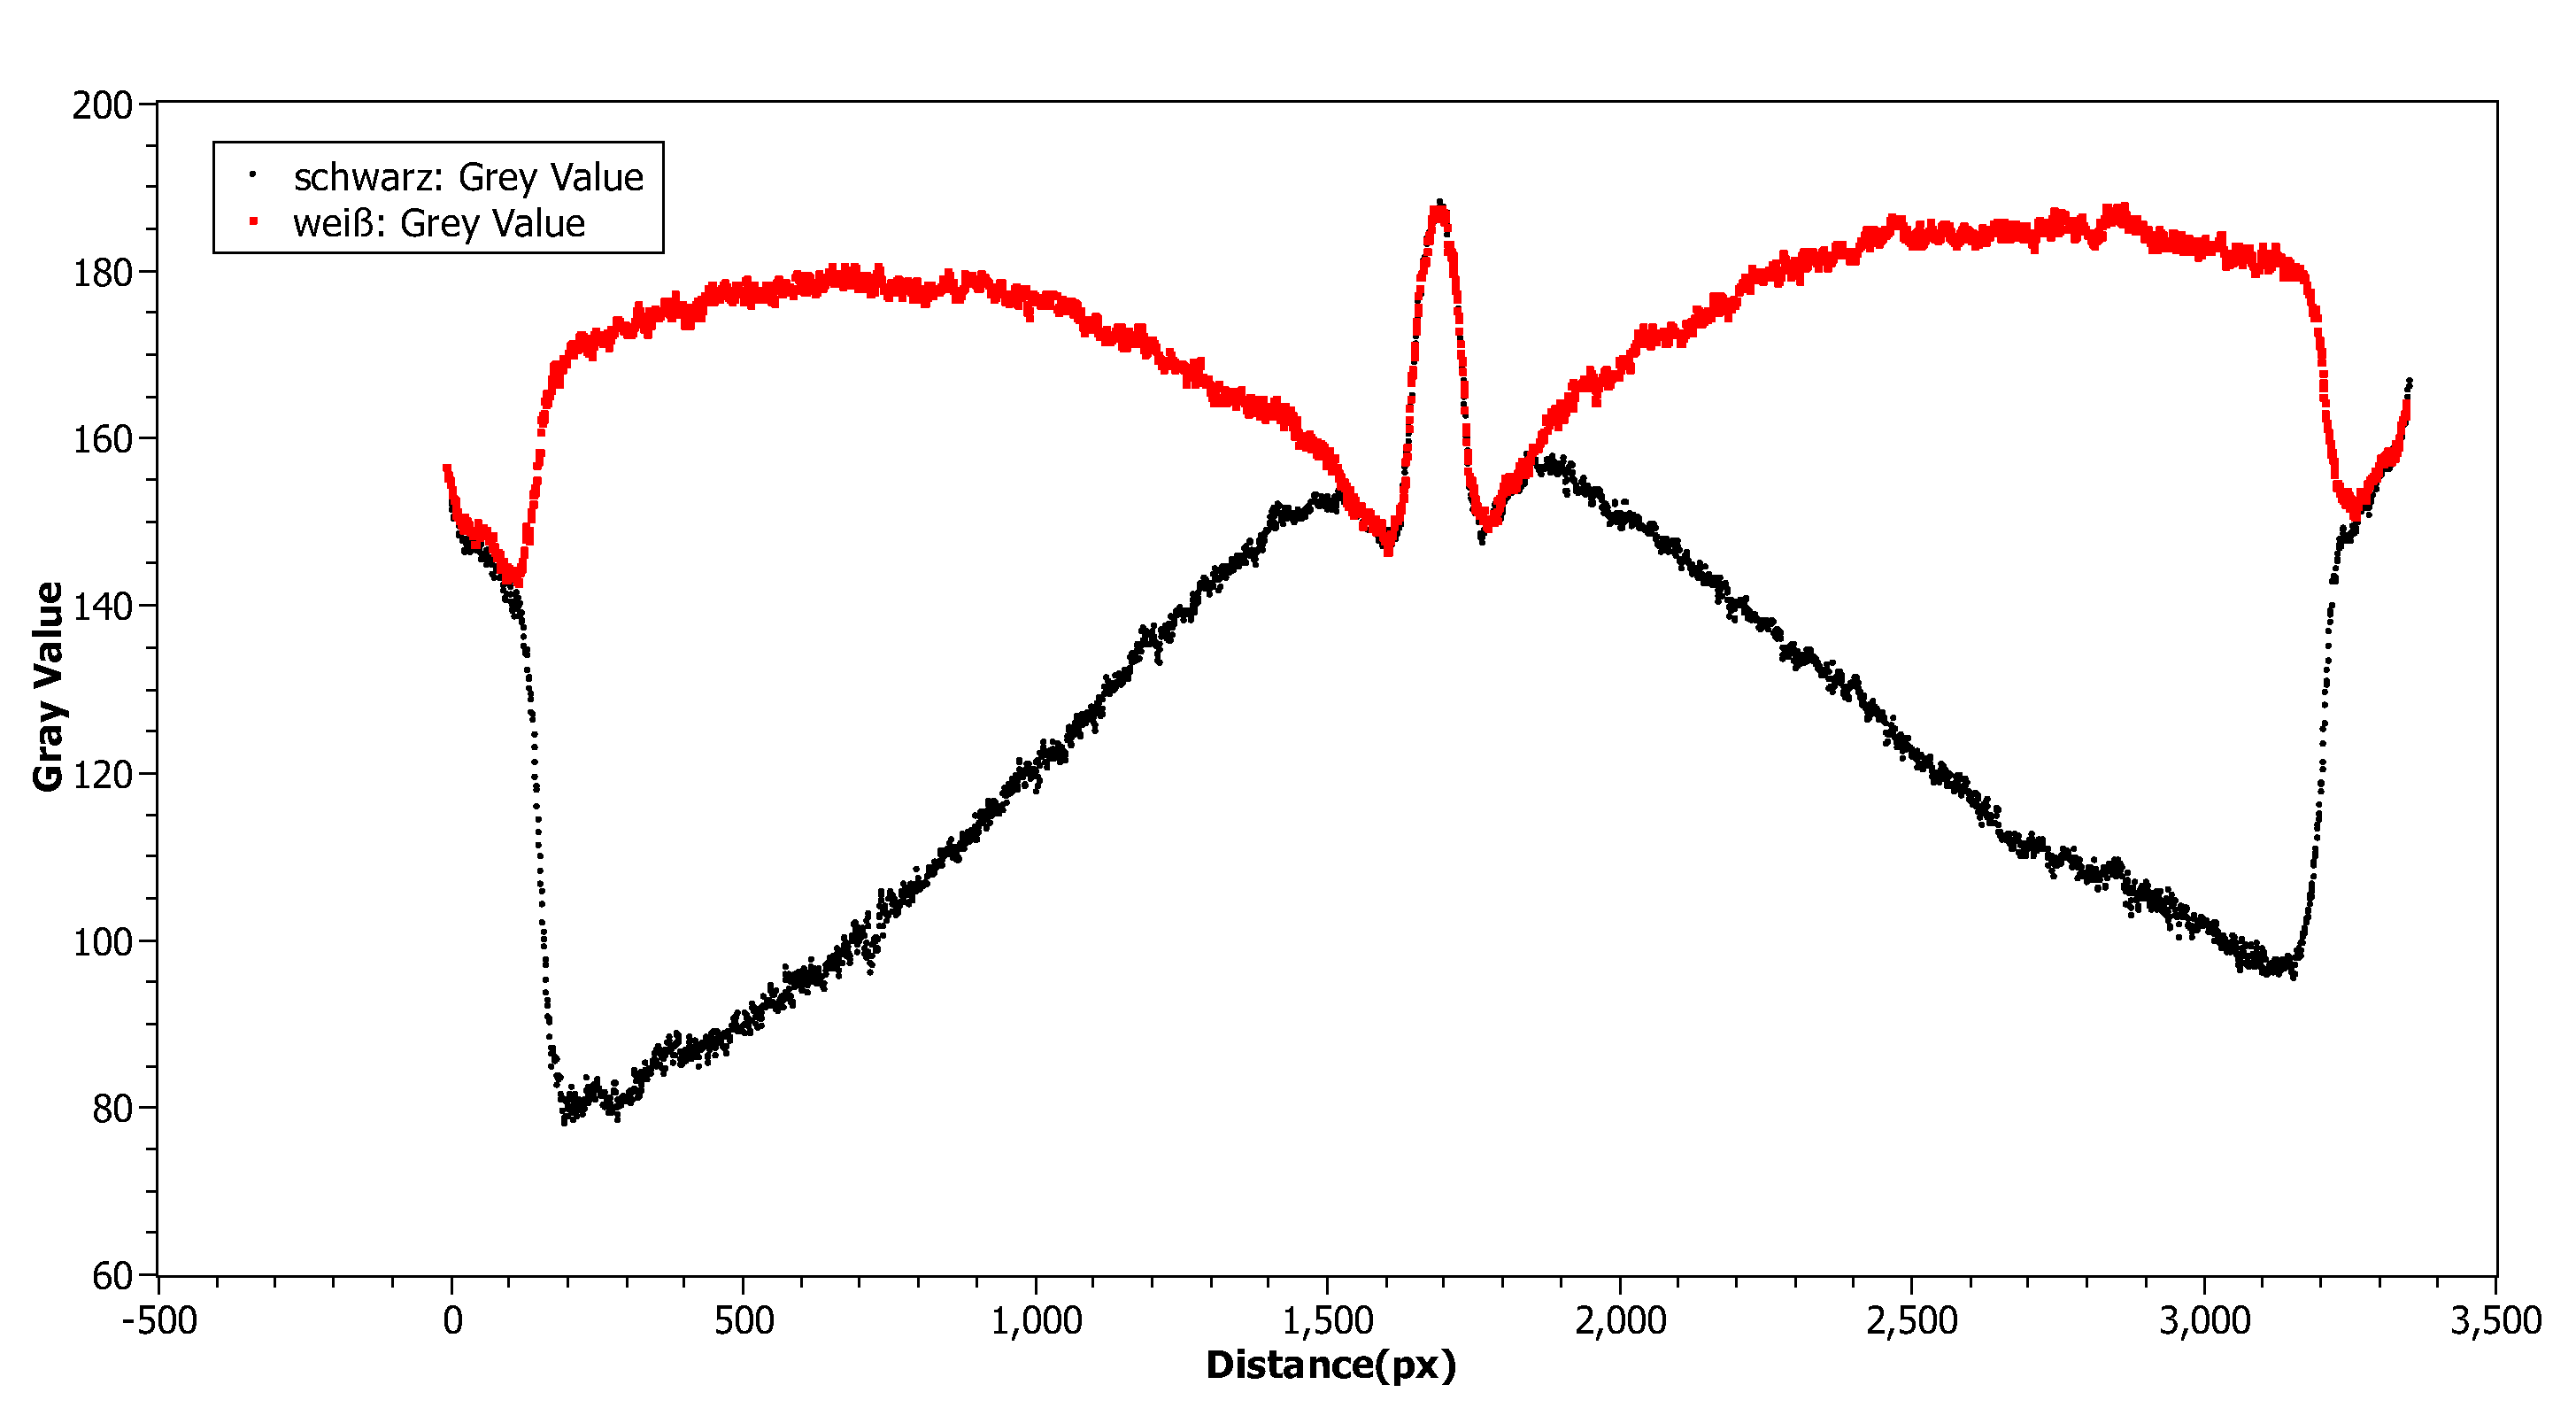
\includegraphics[width=1\textwidth]{fig_lochblende}
		\centering
		\caption{
		Überlagerung der Linienprofile von schwarzem zu schwarzem bzw. weißem zu weißem Bereich des Siemenssterns bei Fotografie durch Lochblende.
		Hier ist als Beispiel das Profil bei einer Blende mit einem Durchmesser von \SI{3,75}{mm} für den Siemensstern nahe der Mitte des Fotos dargestellt.
		Abgelesen werden der Abstand der Schnittpunkte der Profile in der Mitte sowie die Breite des Maximums in der Mitte.
		Ein Wert von 0 entspricht dabei Schwarz und ein Wert von 255 entspricht Weiß.
		}
		\label{fig_lochblende_profil}
		\centering
	\end{figure}
	
	Durch analoge Berechnungen wie oben ergibt sich für die Auflösung in Linienpaaren $l = \SI{0.28\pm 0.05}{mm}$.
	
	\subsubsection*{Größe der Blendenöffnung}
	Die Belichtung beim Fotografieren ergibt sich aus der Blendenöffnungsfläche und der Belichtungszeit:
	\begin{equation}
		B = A \cdot t_\text{B} = \frac{\pi d^2}{4} \cdot t_\text{B}
	\end{equation}
	Um die Belichtung für verschiedene Blenden konstant zu halten muss die Belichtungszeit vervierfacht werden, wenn sich der Blendendurchmesser halbiert.
	In \cref{ss_einzellinse} wurden für jede Linse eine Belichtung von \SI{4,42}{mm^2/s} gewählt.
	Da das Bild der der Lochblende ähnlich belichtet ist wie die der Einzellinsen, kann von einer gleichen Belichtung ausgegangen werden.
	Lässt man sich von ImageJ Grau-Weiß-Histogramme ausgeben, zeigt sich jedoch eine Abweichung in dem Grauton der reinen weißen Flächen.
	Da dies durch den geänderten Abstand zum Testchart verursacht wird, kann nicht von der gleichen Belichtung ausgegangen werden und diese muss mit einem Fehler abgeschätzt werden.
	Außerdem variiert der Mittelwert des Histogramms je nach gewähltem (möglichst großem) weißen Segment des Bilds durch die ungleichmäßige Beleuchtung der Lampe zwischen 120 und 170 (0=schwarz, 255=weiß).

	Deshalb wird die Belichtung $B$ mit \SI{4+-2}{mm^2/s} abgeschätzt und es folgt mit einer Belichtungszeit von $t_\text{B}=\SI{6}{s}$:
	\begin{equation}
		d = \sqrt{\frac{4B}{\pi t_\text{B}}} = \SI{0,9+-0,3}{mm}
	\end{equation}
	\begin{equation}
		u(d) = \sqrt{\frac{1}{\pi t_\text{B}B}}u(B)
	\end{equation}

	
	\subsubsection{Diskussion}
		Das Abschätzen des Durchmessers der Lochblende mit dem Auge ergibt einen Wert in der Größenordnung von einem Millimeter.
		Dies deckt sich erwartungsgemäß mit dem experimentellen Befund von \SI{0,9\pm 0,3}{mm}.
		
		Weiterhin lässt sich sagen, dass die Lochblende eine schlechtere Auflösung ergibt als die Einzellinse bei Blendendurchmessern, die kleiner oder gleich \SI{15}{mm} sind.
		Dies entspricht der Erwartung.
	\section{Schlussfolgerung}
	Zusammenfassend lässt sich sagen, dass sowohl Auflösung als auch Schärfentiefe verschiedener Objektive gemessen werden konnte.
	Dabei wurde zunächst die Schärfentiefe eines Nikkor-Objektiv bei verschiedenen Blendenzahlen untersucht.
	Der Vergleich von subjektiv wahrgenommener Schärfentiefe mit der theoretisch erwarteten führt zu der Schlussfolgerung, dass für die Durchmessergrenze der Zerstreuungskreise ein geringerer Wert verwendet werden sollte.
	
	Als nächstes wurde die Auflösung in Linienpaaren einer Einzellinse mit Blenden verschiedener Durchmesser ermittelt.
	Dabei konnte erwartungsgemäß gezeigt werden, dass ein linearer Zusammenhang zwischen Halbwertsfrequenz aus einer MTF-Kurve und dem Kehrwert der Auflösung in Linienpaaren besteht.
	Dass der Linearitätsfaktor der Anzahl von Pixeln pro Millimeter entspricht, kann lediglich in der Größenordnung gezeigt werden.
	
	Zuletzt wurde eine Lochblende als Objektiv verwendet und die Auflösung sowie die Halbwertsfrequenz bestimmt.
	Außerdem konnte hier bestätigt werden, dass sich der Lochdurchmesser zumindest größenordnungsmäßig aus der benötigten Belichtungszeit bestimmen lässt.
	Um die Güte dieser Messmethode konkreter prüfen zu können, müsste z.B. durch Triangulation mit einem Laser und einem elektronischem Bildwandler der Durchmesser der Lochblende bestimmt werden, und so einen deutlich präziseren Vergleichswert zu haben.
	\printbibliography
\end{document}
